\documentclass{thesis-ekf}
%\documentclass[twoside]{thesis-ekf}
%\documentclass[colorlinks]{thesis-ekf}
\usepackage[T1]{fontenc}
\PassOptionsToPackage{defaults=hu-min}{magyar.ldf}
\usepackage[magyar]{babel}
\usepackage[utf8]{inputenc}
\usepackage{listingsutf8,xcolor,caption,graphicx,amsmath,amssymb,amsthm, url, hulipsum, hyperref, minted}
\footnotestyle{rule=fourth}

\graphicspath{{./pictures/}}

\newtheorem{tetel}{Tétel}[chapter]
\newtheorem{lemma}[tetel]{Lemma}
\theoremstyle{definition}
\newtheorem{definicio}[tetel]{Definíció}
\newtheorem{feladat}[tetel]{Feladat}
\theoremstyle{remark}
\newtheorem{megjegyzes}[tetel]{Megjegyzés}
\newtheorem*{megoldas}{Megoldás}

\begin{document}
\logo{
\includegraphics[width=8cm]{eke-logo.pdf}}
\institute{Matematikai és Informatikai Intézet}
\title{Kliens-szerver kommunikáció\\Android platformon}
\author{Balajti-Tóth Kristóf\\Programtervező Informatikus BSc}
\supervisor{Tajti Tibor\\Tanársegéd}
\city{Eger}
\date{2019}
\maketitle
\tableofcontents
\listoffigures
\renewcommand\listoflistingscaption{Forráskódok jegyzéke}
\listoflistings

\chapter*{Bevezetés}
\markboth{Bevezetés}{Bevezetés}
A szoftver fejlesztés egy nagyon komplex folyamat és rengeteg részletre oda kell figyleni.
Az elkészült programnak hatékonynak, hibamentesnek és gyorsnak kell lennie. Természetesen, mindezt határidőn belül kell teljesíteni.
Sajnos a biztonság nem egy első számú szempont egy megrendelő szemében, csak akkor ha már valami baj történt.
Inkább a gyorsaságon és a folyamatok automatizálásán van a hangsúly, ezért nem  meglepő, hogy a fejlesztés életciklusának tervezési szakaszában kevés figyelem fordul a szoftver biztonságossá tételére.

A statista.com \cite{statista} kutatása szerint 2020-ra több mint 4.78 billió telefon lesz használatban.
Ezzel a cégek is tisztában vannak és tudják, hogy ha még több emberhez szeretnék eljuttatni a szolgáltatásukat, akkor rendelkezniük kell saját mobilos app~-al.

A mobilos eszközöket célzó támadások száma hatalmas ütemben nő. Mindez azért lehetséges, mert figyelmen kívül marad a ,,secure coding''-nak nevezett gyakorlat.
Egy alkalmazásnak a sebezhetőségét különböző támadási vektoron is ki lehet aknázni.
Az elején, bennem többek között az a kérdés merült fel, hogy honnan tudható hogy ez alkalmazás ebezhető-e vagy sem.egy kérdés merült fel.
Honnann tudhatom, hogy egy adott alkalmazás sebezhető-e vagy sem és ha igen milyen súlyos a hiba.
A leghatékonyabb módszer ha megpróbáljuk visszafejteni az alkalmazást forráskódra.
Ezt angolul ,,reverse engineering''-nek nevezik.
A visszaállított fájlok olvashatósága nem lesz tökéletes, főleg ha obfuszkált \footnote{Az obfuszkáció célja röviden, hogy megnehezítse a visszafejtett kód olvashatóságát.} kóddal állunk szemben, de egy tapasztalt szem így is kitudja szúrni a gyakori hibákat.

A szakdolgozatomban Android platformra készült alkalmazások forrás fájlokká való visszaállításáról írok, valamint bemutatom hogyan valósítható meg a kliens-szerver kommunikáció egy REST API és egy Android platforma készült kliens segítségével.
Szó lesz arról, hogy hogyan tudunk fájlokat feltölteni/letölteni és értesítésekkel operálni.
A felhasználó egy egyszerű autentikáció után képes lesz \emph{.apk} fájlok feltöltésére, letöltésére és az elkészült projektben való navigálásra.
Hosszabb ideig tartó folyamatok állapotáról és elkészültéről értesítést kap és lehetősége lesz a forráskód alkalmazáson belüli megtekintésére és megosztására.
A projektet ,,Reverse Droid''-nak neveztem el.

\chapter{Fejlesztői környezetek}\label{kornyezetek}

\section{Android Studio}

Az Android Studio jelenleg az egyetlen jól támogatott és minőségi fejlesztői környezet Android fejlesztéshez.
Régebben sok panaszt hallottam az emulátorára, hogy nagyon lassú és körülményes a használata.
Mára már egy pillanat alatt lehet futtatni a programunk és abszolút kényelmes lett a használata.
Az emulátor állapota menthető, ezáltal indításkor ott folytathatjuk ahol abba hagytuk. Azon kívül, hogy használatával több különböző eszközön tesztelhetjük az alkalmazásunk, lehetőséget ad a szenzorok, hálózati és GPS kapcsolat szimulálására. 
Rendelkezik APK elemzővel, vizuális felhasználó felület szerkesztővel és intelligens kód szerkesztővel is.
Az egyik kedvenc funkcióm a valós idejű profilozó, ami segítségével megtudjuk nézni valós időben, milyen erőforrásokat használ az alkalmazásuk.
Ez különösen hasznos, ha megakarunk találni egy memória szivárgást vagy egy olyan részt, ami a kelleténél jobban meríti az akkumulátorunk.
Említésre méltó még a flexibilis build rendszere is, a Gradle. Használatával megtehetjük, hogy külön build típusokat hozzunk létre a különböző eszközökre.
Az \emph{instant run} funkció segítségével egyből tudjuk futtatni a kódban véghez vitt kisebb változtatásokat, anélkül hogy újraindítanánk az Activity~-t vagy újra buildelnénk az egész projektet és új APK~-t telepítenénk.
\cite{androidstudio}

% https://developer.android.com/studio/features.html

\section{Pycharm Professional Edition}

A PyCharm is egy IDE \footnote{Integrated Development Environment (integrált fejlesztői környezet)}, mint az Android Studio.
Dolgozhatunk webes technológiákkal vagy mesterséges intelligenciával, a PyCharm megfelelő választás lehet bármilyen területen programozó számára.
A Pycharm mögött is a \emph{Jetbrains} cég áll. Ezt azért fontos megemlíteni, mert már 15 éve azon dolgoznak, hogy a legjobb és leghatékonyabb fejlesztői környezetek állítsanak elő.
Véleményem szerint ez sikerült is nekik. Az Android Studio-n és a Pycharm-on  is látszik, hogy minőségi termékek és rengeteget segítenek a fejlesztők mindennapjaiban.
Én a \emph{PyCharm Professional Edition}-t használtam, amihez a diákok ingyenesen hozzájuthatnak.
Mivel adatbázissal is dolgoznok, ezért a \emph{Community Edition} nem lett volna megfelelő.
Nem csak az adatbázis támogatást nyújt, hanem webes keretrendszer támogatást és profilozót is.
A távoli fejlesztés funkció is rendkívül praktikus. A fejlesztés közben egyszerűen tudtam feltölteni a szerverre a változtatásaimat.
A verzió kezelőknek is egyesített felületet nyújt, amivel jelentős időt spórolhatunk meg.
Ez a lehetőség mindkettő fejlesztői környezetben elérhető.\cite{pycharm}

% https://www.jetbrains.com/pycharm/features/
% https://www.jetbrains.com/company/

\section{Postman}

Jelenleg a Postman a legnépszerűbb API\footnote{Application Programming Interface} tesztelésben használt eszköz.
A Postman kollekciók futtatható leírásai egy API-nak és sarok kövei a Postman beépített eszközeinek.
Ezeknek a beépített eszközöknek köszönhetően futtathatunk hálózati kéréseket, teszteket, debuggolhatunk és csinálhatunk mock szervereket is.
Ráadásul automatizáltan futtathatjuk a teszteket és egyszerűen elkészíthetjük és publikálhatjuk az API dokumentációját.
Én csak dokumentáció készítésre és a végpontok tesztelésére használtam. Ettől természetesen sokkal több lehetőség rejlik benne.
A \ref{postman} képen látható egy kérés, ami tartalmaz egy \emph{Authorization Header}-t.
Attól függően, hogy helyes-e a felhasználó név és jelszó páros a szerver visszaad egy választ JSON formátumban, amit a kép alján láthatunk.

\begin{figure}[!h]
	\centering
	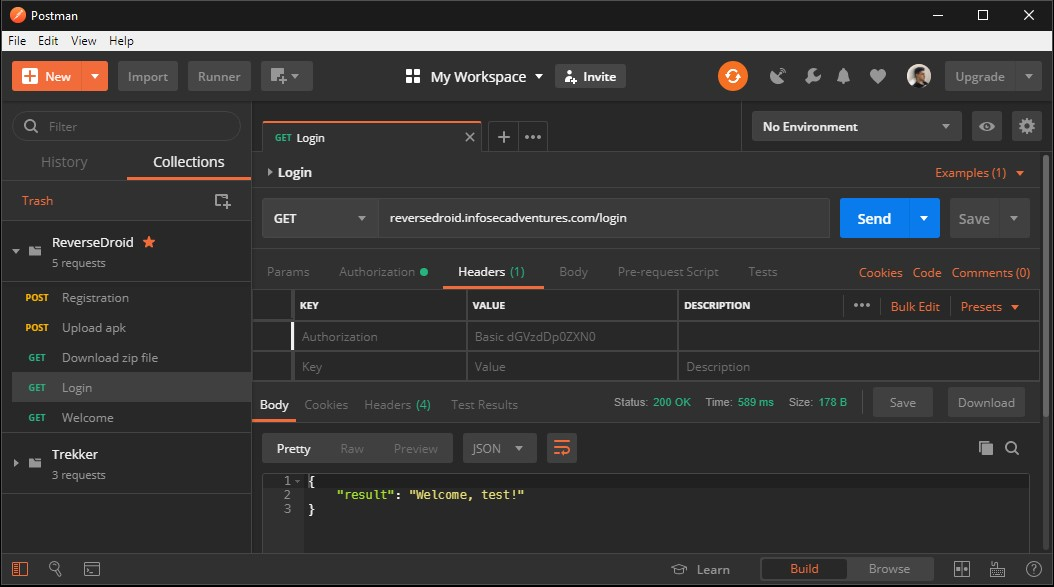
\includegraphics[width=15cm]{pictures/postman}
	\caption{Egy GET kérés és válasz a Postman alkalmazásban.}
	\label{postman}
\end{figure}

\chapter{Platformok}\label{platformok}

\section{A szerver kiválasztása és felépítése}

Olyan szerverre volt szükségem, ami nem túl költséges, de mégis megfelelően testreszabható és gyors tárhelyet biztosít.
A választásom a Digitial Ocean felhő szolgáltatására esett. Az oldal felületén lehetőségünk van több, úgynevezett \emph{droplet}-et létrehozni, amik nem mások mint virtuális szerverek. 
Megadhatjuk milyen disztribúciót szeretnénk telepíteni, jelen esetben én az Ubuntu Linux 18.10-es verzióját választottam.

Szerencsére nem kellett új domain nevet vásárolnom, mert már rendelkeztem egyel.
A domain egyébként a \emph{Namecheap} oldalon van beregisztrálva.
Annyi volt a dolgom, hogy egy új aldomaint kellett készítenem a projekt számára.
Miután feltelepült a Droplet hozzárendeltem az IP\footnote{Internet Protocol} címét az előbb elkészített aldomainhez.
Ezzel biztosítottam, hogy domain név alapján is elérhető legyen a szerver.
Körülnéztem a konkurens cégek által nyújtott szolgáltatások között is, de én úgy láttam, hogy egyik se éri el azt az ár-érték arányt, amit a \emph{Namecheap} nyújt. 

Habár nagyon egyszerű volt a folyamat, az elkészült projektben mégsem ezt a folyamatot választottam, hanem a Digital Ocean által nyújtott ,,one-click apps'' menüben egyszerűen kiválasztottam a Docker alkalmazást és az elkészült képfájlt ezen futtattam. 
Így automatizálva a szerver telepítésének folyamatát és megspórolva a Docker telepítését és konfigurálását.
Erről még a \nameref{szerveren_hasznalt_technologiak} fejezet \nameref{docker} alfejezetében bővebben írok.

\section{Mobil platform választása}

A mobilos operációs rendszerek közül az Androidot választottam. Bevallom őszintén, nem volt nehéz a döntés. 
Android platform rengeteg olyan lehetőséget biztosít, amivel a többi platform nem szállhat versenybe.
Itt gondolok az egyszeri és nem megújuló fizetésre a fejlesztői fiókért, valamint az iOS-el ellentétben a fejlesztői környezete elérhető mind a három fő operációs rendszerre (Linux, macOS, Windows).
Számomra ezek elég nyomós érvek voltak, ezért döntöttem úgy, hogy Android platformra fog először elkészülni a program.
A Windows Phone a Microsoft cégnek volt egy próbálkozása, ami végül kudarcba fulladt, ezért ez az opció nem jöhetett szóba.

A többi mobilos operációs rendszerrel ellentétben az Android nyílt forráskódú és a piac jelentős részét uralja.
Engem különösen megfogott az általa nyújtott szabadság és testre szabhatóság.
Az iOS ezzel ellentétben arról híres, hogy egyszerű és megbízható a használata.
Viszont jelen vannak olyan megkötések, amik mind a végfelhasználókat és mind a fejlesztőket limitálják.
Gondolok itt a minimális testre szabhatóságra és a nagy részt zárt forráskódra.
Itt most nyilván nem szeretném részletezni, hogy melyik operációs rendszer a jobb vagy éppen rosszabb, mert mindegyik rendszernek megvan az előnye, illetve a hátránya.
Inkább csak a személyem érveimet és tapasztalataimat sorakoztatom fel, amik alapján platformot választottam.


Fontos megemlíteni, hogy az Android rendszer nem csak mobil telefonokban terjedt el.
Jelen van az okos televíziókban (Android TV), autókban (Android Auto), okos órákban (Wear OS) és IoT\footnote{Internet of Things}-ben is (Android Things).
Ezek az Android által úgymond eredmények annak is köszönhetőek, hogy a Google felvásárolta az Android céget és azóta ők tartják karban.

Természetesen nem csak jó tulajdonságokkal rendelkezik, hanem bizony van néhány hátránya is.
Ide tartozik például a gyártóktól függő frissítések. Tegyünk fel, hogy új biztonsági rést fedeztek fel az Android operációs rendszerben.
A Google általában ezekre meglehetősen gyorsan reagál és néhány napon belül frissítést ad ki az eszközeire (Nexus, Pixel).
Azoknak a gyártóknak akiknek saját testre szabott rendszerük van, jóval tovább tart orvosolni a hibát.
Ez az időtartam a mai napig hónapokban mérhető, de persze ez függ az adott cégtől és a hiba súlyosságától. 

Számomra ezek voltak a legnyomósabb érvek a rendszer kiválasztásában.
A mai napig úgy gondolom, hogy ebben a platformban van a legnagyobb potenciál a fejlesztők és felhasználók számára egyaránt.

\chapter{Felhasznált technológiák}\label{technologiak}

\section{Verzió kezelés}

Egy verzó kezelő rendszer képes kezelni egy fájl vagy akár több fájl módosításait olyan módon, hogy lehetőségünk legyen időben ,,visszamenni'' és megnézni egy fájl bizonyos verzióját.
A Linux kernel forráskódja óriási méretű és a Git verzió kezelőt használják a fejlesztéshez.
Ez azért érdekes, mert nagyon sok ember dolgozik egy óriási kódbázissal és a Git mégis képes hatékonyan kezelni a változásokat.
A alábbi listában látható, hogy miért bíznak meg benne egy ilyen nehéz feladat esetében és hogyan teljesíti a Git minden elvárásukat:

\begin{itemize}
	\item Atomosság
	\item Teljesítmény
	\item Biztonság
\end{itemize}

Az atomosság biztosítja, hogy az adatok ne vesszenek el és ne történjen verzió eltérés részlegesen befejezett műveletek miatt.
A gyorsasága mellett nem használ fel jelentős mennyiségű tárhelyet, ellentétben a többi verzió kezelő rendszerrel.
Ha Git-et használunk biztosra mehetünk, hogy senki sem módosítja a fájlok tartalmát. Ez a SHA-1 kivonatolásnak köszönhető.\cite{git}

A fentiek fényében nyilvánvaló, hogy a Git mellett döntöttem, ami széles körben elterjedt a szoftver fejlesztők között.
A Git egy ingyenes és nyílt-forráskódú elosztott verzió kezelő rendszer. Úgy készült, hogy gyorsan és hatékonyan tudjon kezelni kis és nagy projekteket is egyaránt.
Már a project kezdetekor készítettem egy privát Github repository-t, hogy nyomon tudjam követni a változtatásaimat és esetleges hiba esetén visszaállítani egy korábbi verzióra.

A Github nem összetévesztendő a Git-el, mert a Git a forráskód változtatásainak kezelésére szolgál (lokálisan), a Github pedig egy tárhelyet nyúlt a verzió kezelt könyvtárak és fájlok tárolására.
A projekt fejlesztése alatt több gépről dolgoztam és Github a segítségével biztosítani tudtam, hogy mindenhol elérjen a projektek legfrissebb változtatásait.
Lényegében egy központi szerverként szolgált számomra.

\section{Folyamatos integrálás}

A folyamatos integrálás egy szoftver fejlesztési gyakorlat, ahol a csapat tagjai sűrűn integrálják a munkájukat általában napi rendszerességgel. 
Ez naponta több integrációhoz vezet. Pontosabban megfogalmazva a folyamatos integrálás egy extrém programozási gyakorlat.
A folyamatos integrálás arról szól, hogy ha egy feladat elkészült akkor azt egyből beintegráljuk a rendszerbe.
Minden integráció hitelesítve van egy automatikus build rendszer által (egység tesztekkel együtt) annak érdekében, hogy minél hamarabb észrevegyük az integrációs hibákat.
A beintegrálás után természetesen minden egység tesztnek sikeresen le kell futnia.
Sok csapat úgy gondolja, hogy ez a megközelítés jelentősen kevesebb integrációs problémához vezet és meggyorsítja a fejlesztés menetét.\cite{continuous_integration}

Több nagy cég is a CircleCi szolgáltatását használja a folyamatos integráláshoz, ilyen például a \emph{Facebook}, \emph{Spotify} és a \emph{GoPro}.
A CircleCi összeköthető a Github-al, így kényelmesen tudjuk csatolni az ott tárolt projektjeinkket.
A konfigurációs fájl létrehozása pedig végtelenül egyszerű, ha követjük a dokumentációt.
A \ref{circleci} képen látható, hogy minden egyes változtatáskor lefutnak a tesztek.
Ezek a tesztek minden alkalommal egy tiszta konténerben vagy virtuális gépen futnak.
Jelen esetben az Android program egy Docker konténerben fut, aminek a neve \emph{circleci/android:api-28-alpha}.
Az eredményről mindig értesítést kapunk, így egyből tudhatjuk azt is, ha egy build nem volt sikeres.

\begin{figure}[!h]
	\centering
	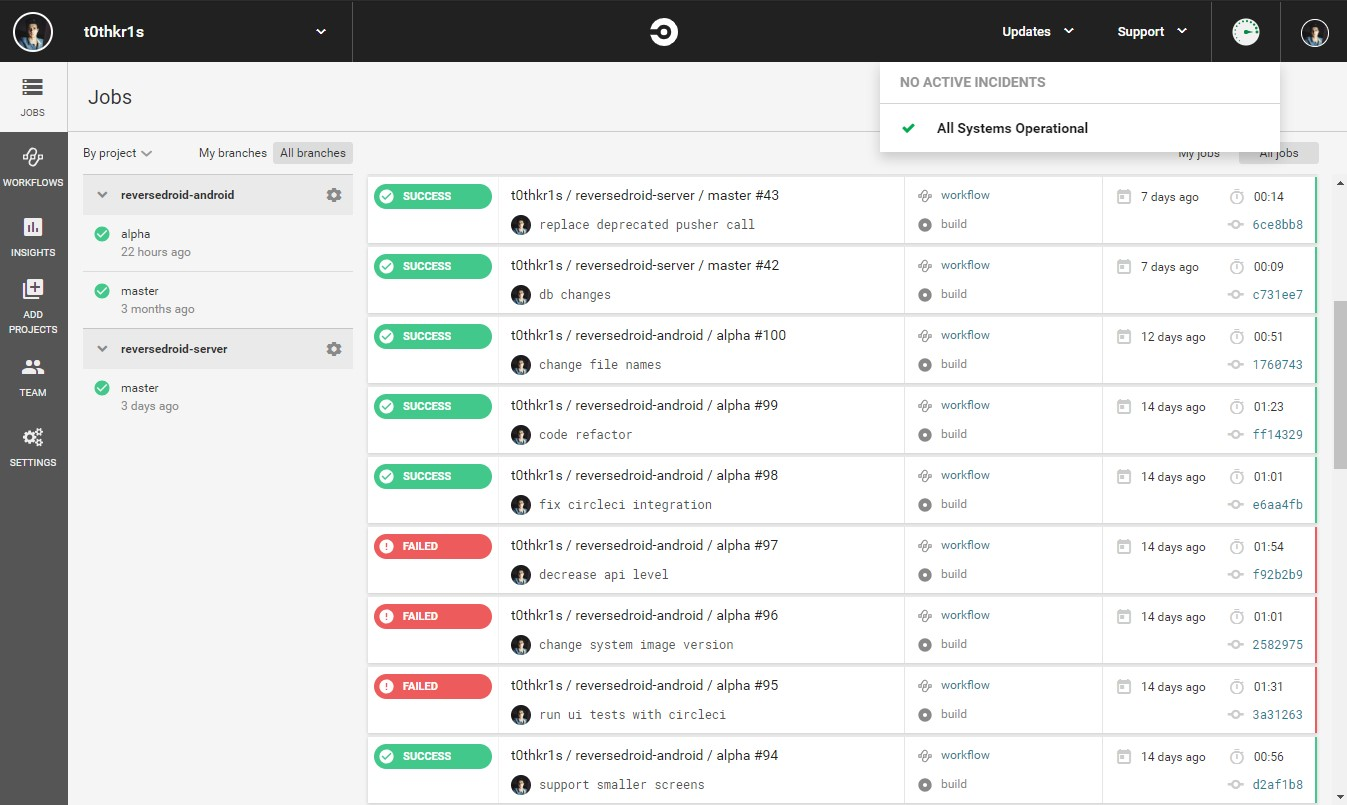
\includegraphics[width=15cm]{pictures/circleci}
	\caption{Project buildek követése a CircleCi felületén.}
	\label{circleci}
\end{figure}

\newpage

\section{Szerveren használt technológiák}\label{szerveren_hasznalt_technologiak}

\subsection{Flask}

A szervert a Flask webes mikro keretrendszer felhasználásával készítettem el.
Attól, hogy mikro keretrendszer még nem jelenti azt, hogy kevesebb tud mit a többi keretrendszer.
Erős alapot nyújt az alapvető szolgáltatásokkal, miközben a kiegészítők nyújtják a többit.
Azzal a lehetőséggel, hogy kitudjuk választani magunknak a kiegészítő csomagokat, képesek vagyunk egy olyan programok felépíteni, ami pontosan azt tartalmazza amire szükségünk van és nem tartalmaz semmi fölöslegeset.

A Flask nem támogatja natívan az adatbázis elérést, web formok validálását, felhasználói autentikációt és egyéb magas szintű feladatokat.
Ezek és más egyéb kulcs szolgáltatások, amikre egy webes applikációnak szüksége van kiegészítőkön keresztül elérhető.
Fejlesztőként lehetőségünk van egyesével kiválogatni vagy éppen magunktól megírni azokat a kiegészítőket, amik az aktuális projekthez kellenek.
\cite{flask}

Úgy gondolom, hogy sokkal hatényobban programot lehet írni, ha csak azt építjük bele a szoftverbe, amire tényleg szükségünk van.
Nekem csak kettő kiegészítőre volt szükségem, mivel a többi funkcionalitást alapból nyújtja a keretrendszer.

\subsubsection{Flask-Testing}

Az egyik ilyen a ,,Flask-Testing'' csomag, amire az egység tesztek miatt volt szükségem.
Segítségével rendkívül egyszerűen és hatékonyan tudjuk tesztelni az alkalmazásban található végpontokat.
Használata számomra nagyon könnyű volt és a dokumentáció minden felhasználási esetre kitért és lehetővé tette, hogy kényelmesen teszteljem a JSON válaszokat.
A dokumentáció azt ajánlja, hogy tegyünk minden tesztet egy nagy fájlba, mert így kényelmesen tudjuk egyszerre futtani őket.

\subsubsection{Flask-Bcrypt}

Mivel alapból a Flask keretrendszer nem biztosít titkosítás, keresnem kellett egy külső megoldást.
A másik ilyen csomag amit felhasználtam, a ,,Flask-Bcrypt'' volt.
Nagyon rossz gyakorlat, ha a jelszavakat titkosítás nélkül tároljuk az adatbázisban.
Ennek elkerülése érdekében választottam a bcrypt algoritmust szolgáltató csomagot, ami kifejezetten erre a célra készült.

\subsection{SQLite}

Az SQLite egy nyílt forráskódú szoftver csomag, ami relációs adatbázis kezelő rendszert biztosít.
Relációs adatbázis rendszereket arra használjuk, hogy a felhasználó által meghatározott rekordokat nagy méretű táblákban tároljunk.
Az adat tárolás és kezelés mellett, az adatbázis motor komplex lekérdezéseket dolgoz fel.
Néhány meghatározó funkciója az SQLite adatbázisnak:

\begin{enumerate}
	\item
	\begin{description}
		\item[Szerver mentes] Az SQLite-nak nincs szüksége külön szerver folyamatra vagy rendszerre a működéshez. Az SQLite könyvtár közvetlenül kezeli a tárhely fájlokat.
	\end{description}
	\item
	\begin{description}
		\item[Nulla konfiguráció] Ha nincs szerver, nincs konfiguráció sem. Úgy csinálhatunk SqLite adatbázist, mintha fájlt hoznánk létre.
	\end{description}
	\item
	\begin{description}
		\item[Platform független] Az egész adatbázis példány egy darab platform független fájl, ami semmilyen adminisztrációt nem igényel.
	\end{description}
	\item
	\begin{description}
		\item[Önálló] Egy darab könyvtár tartalmazza az egész adabázis rendszert, ami közvetlenül az alkalmazásba integrálódik.
	\end{description}
	\item
	\begin{description}
		\item[Tranzakciós] Lehetővé teszi a biztonságos hozzáférést más szálakból vagy folyamatokból.
	\end{description}
	\item
	\begin{description}
		\item[Kifejezetten megbízható] A SQLite fejlesztői csapata nagyon komolyan veszi a forráskód tesztelését.
	\end{description}
\end{enumerate}

Összességében az SQLite egy funkcionális és fexibilis relációs adatbázis környezet, ami csak minimális erőforrást igényel.
\cite{sqlite}
Nem mellesleg ez a legtöbbet használt adatbázis motor a világon. 
Számtalan alkalmazás használja és Android platformon is ez az alapértelmezett adatbázis.
Ha többet szeretnénk megtudni róla, akkor azt megtehetjük a \url{https://www.sqlite.org/index.html} oldalon.

\subsection{Pusher Beams (Python Server SDK)}\label{pusher_server}

A szerverről való értesítés küldéshez a Pusher Beams SDK\footnote{Software Development Kit}-ját használtam.
A Beams SDK lehetővé teszi, hogy egyszerűen küldjünk push értesítést ,,érdeklődési'' körök alapján és platformtól függetlenül.
Ingyenesen és korlátlanul küldhetjük ezeket az értesítéseket. Erről bővebben olvashatunk a \url{https://docs.pusher.com/beams} oldalon.
Ha kimondottan a szerver oldali python  dokumentációt szeretnénk elolvasni, azt megtehetjük itt: \url{https://docs.pusher.com/beams/reference/server-sdk-python}
A szerver és kliens is oldal implementációja is nagyon egyszerű és jól dokumentált, de ha mégis problémánk támadna az online ügyfélszolgálatuk is végtelenül segítőkész.

Bevallom, amikor implementáltam a szerverről való üzenetküldést nem ment minden simán.
Az volt a probléma, hogy csak azt az értesítést kaptam meg amelyik nem tartalmazott plussz adatot az értesítés címén és leírásán kívül.
Fel kellett keresnem őket, mert hiába követtem a dokumentációkat nem értettem a hiba okát.
Az üzenetemre kifejezetten gyorsan (egy napon belül) válaszoltak és kérték, hogy küldjek több információt.
Hamar kiderült, hogy a problémát az FCM\footnote{Firebase Cloud Messaging} okozza, ami nem engedi, hogy egyszerre küldjünk értesítést és adatot.
Itt kiegészítésként fontos megemlíteni, hogy a Pusher a Firebase Cloud Messaging által küldi az értesítéseket.
Miután rávilágítottak a hiba okára, egyből megoldást ajánlottak és frissítették a dokumentációjukat.
Úgy sikerült kikerülni ezt a limitációt, hogy kettő darab értesítést kell küldeni.
Az első csak magát az értesítést tartalmazza, a második pedig csak az adatok küldéséért lesz felelős.
Természetesen a második értesítésnek nem lesz vizális reprezentációja a kliens oldalon.

% forrás https://docs.pusher.com/beams/reference/server-sdk-python

\subsection{Docker}\label{docker}

A Docker az egy nyílt forráskódú motor, ami automatizálja az alkalmazások üzembe helyezését konténereken belül.
Úgy lett tervezve, hogy egy pehely súlyú és gyors környezetet nyújtson, amiben hatékonyan tudjuk futtatni a kódunk.
Célja még, hogy hordozhatóvá és könnyen buildelhetővé tegye az alkalmazásunk.
Szolgáltatás orientált architektúrára ösztönöz és azt ajánlja, hogy minden konténerben csak egy alkalmazás fusson.\cite{docker}

\subsubsection{Képfájlok}

A konténereinket képfájlokból futtatjuk.
Rétegezett formátumuk van, ami lépésről-lépésre épülnek fel egy sorozat parancs alapján.
Tulajdonságaikat tekintve hordozhatóak, megoszthatóak, tárolhatóak és frissíthetők.
A következő paranccsal tudunk képfájlt készíteni (feltéve, hogy a Dockerfile az aktuális könyvtárban van):

\begin{minted}{bash}
	$ docker build .
\end{minted}

Minden Docker képfájl rendelkezik egyedi azonosítóval.
A példa kedvéért az én képfálom az ,,edd116d82f90''-es azonosítót kapta, de használatkor nem fontos az egészet kiírni.
Megtehetjük azt is, hogy a 9898-as porton futú szolgáltatást a helyi 80-as portra publikáljuk és így futtatjuk.
Ezt a következő paranccsal tehetjük meg:

\begin{minted}{bash}
	$ docker run -p 80:9898 edd11
\end{minted}

\subsubsection{Konténerek}

A konténerek lényegében a futó képfájlok példányai.
Ha elíndítunk egy képfájt és megnyitunk egy új terminál ablakot, akkor az alábbi paranccsal megtekinthetjük a futó konténert.

\begin{minted}{bash}
	$ docker container ls
\end{minted}

A parancs kiírja többek között a publikált portot, a konténerben futó parancsot és a képfájl azonosítóját is.

\subsubsection{Dockerfile}
A szakdolgozatom szempontjából fontos említést tenni a Dockerfile-ról.
Ez egy szöveges dokumentum, ami tartalmazza azokat a parancsokat, amik egy képfájl felépítéséhez szükségesek.
Segítségével bárki automatikusan készíthet egy docker képfájlt.

\subsubsection{Docker Hub}

A Docker Hub biztosítja azt a platformot, ahol bárki kereshet és megoszthat konténereket.
Kézzel nagyon körülményes lett volna a képfájl verzióinak követése és publikálása, ezért igénybe vettem a Docker Hub szolgáltatását.
Ez a szolgáltatás nem más, mint az automatikus buildek készítése.
A Docker Hub képes külső forráskódból képfájlt készíteni és azt publikálni.
Összetudjuk csatolni a Github projektjeinket a Docker Hub-al. 
Ezzel hozzájárulva ahhoz, hogy minden egyes változtatásnál a Docker Hub újra buildelje a képfájlt és publikálja a frissített verziót.

\begin{figure}[!h]
	\centering
	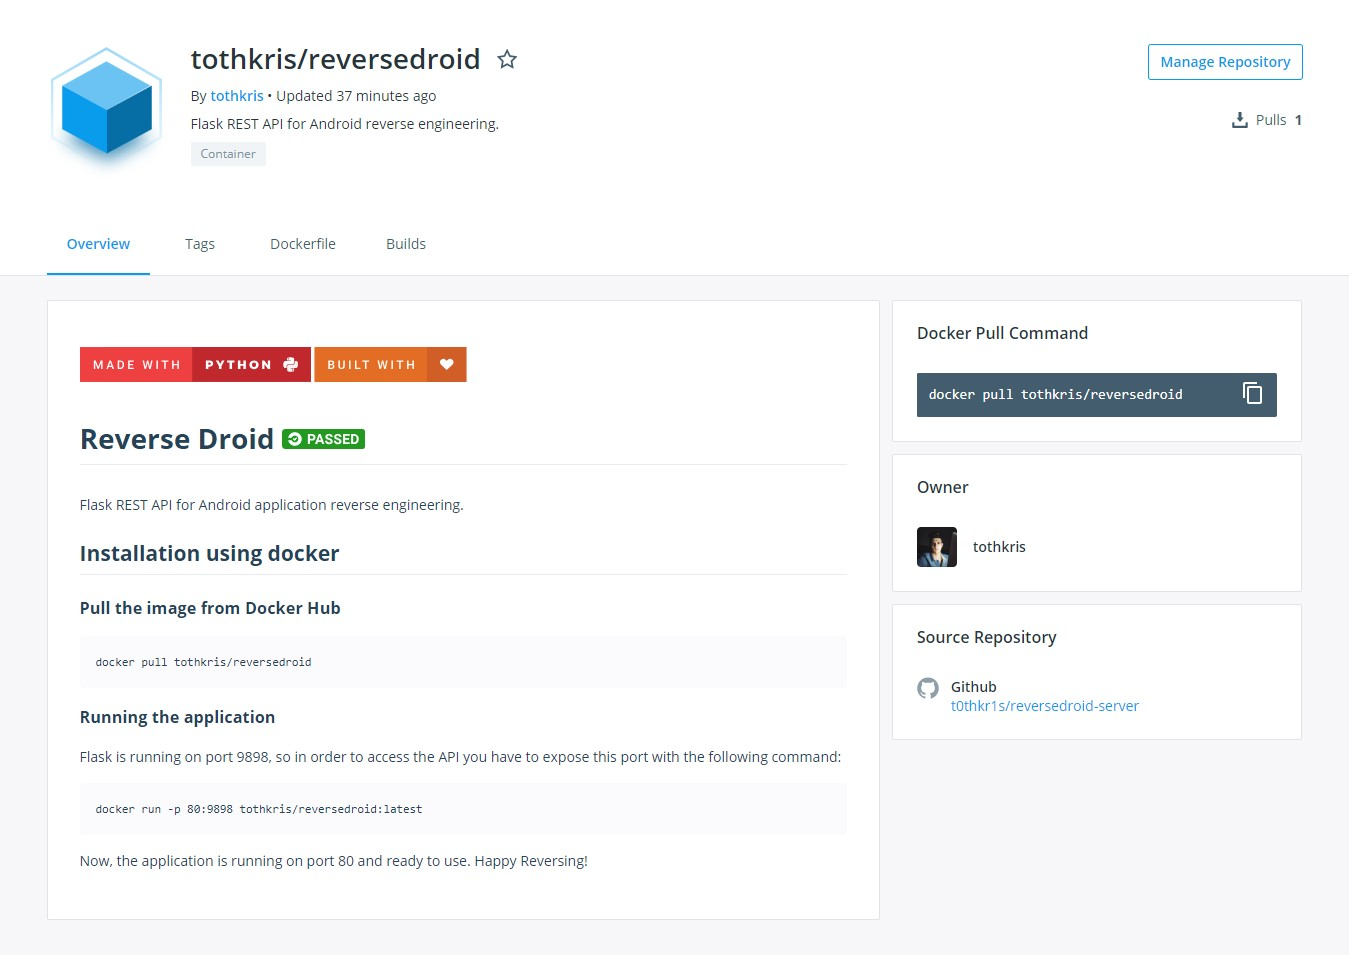
\includegraphics[width=15cm]{pictures/docker_hub}
	\caption{Az applikáció Docker Hub-on is elérhető.}
	\label{dockerhub}
\end{figure}

\subsection{Apktool}

Az Apktool egy olyan eszköz, aminek a segítségével vissza tudjuk fejteni a harmadik féltől származó, zárt forrású, bináris Android alkalmazásokat.
Majdnem eredeti az állapotukba tudja dekódolni a forrásokat és újra buildeni őket néhány módosítással.

Funkciók:

\begin{itemize}
	\item Források visszaállítása majdnem eredeti formájukba
	\item Újra buildelése a dekódolt forrásoknak bináris APK/JAR fájlba
	\item Smali kód debuggolás
\end{itemize}

Az eszköz letölhető a \url{https://github.com/iBotPeaches/Apktool} oldalról.

\subsection{dex2jar}

Android .dex és .class fájlokkal való dolgozáskor kulcs szerepet játszott a \emph{dex2jar}.
Jelen esetben nem csak egy programról beszélünk, mert valójában több eszközt foglal magába.
Az Android telepítő fájl kitömörítése után, az alkalmazás forráskódja egy \emph{classses.dex} fájlban található meg.
Ez a fájl byte kódot tartalmaz az ART\footnote{Android Runtime} számára és ezt kellett átalakítani .jar formátumba, amivel már a decompiler dolgozni tud.
Az eszköz letölthető a \url{https://bitbucket.org/pxb1988/dex2jar} oldalról.

\subsection{JSON}

A JSON\footnote{JavaScript Object Notation} egy platformok közötti adatátvitelre szolgáló formátum.
Az adatátviteli formátum egy olyan szöveges formátum, amit különböző platformok közötti adat cserére használnak.
Egy másik széles körben használt adatátviteli formátum az XML\footnote{Extensible Markup Language}.
Ezek biztosítják a nagyon eltérő rendszerek közötti adatváltást.
A JSON egy olyan formátum, amin megegyeztek ezek a rendszerek adat kommunikáció céljából. \cite{json1}
Kettő struktúrára épül:

\begin{enumerate}
	\item
	\begin{description}
		\item[Kulcs-érték párok] Ez a koncepció nagyon elterjedt a számítástechnikában és több programozási nyelvben van megfelelője. 
	\end{description}
	\item
	\begin{description}
		\item[Listába rendezett értékek] A legtöbb nyelvben megfelel a tömböknek, vektoroknak és listának.
	\end{description}
\end{enumerate}

Ezek olyan univerzális adatszerkezetek, amiket gyakorlatilag minden programozási nyelv támogat ilyen vagy olyan formában.
Ésszerűnek tűnik tehát, hogy az az adatformátum, amelyet programozási nyelvek kommunikációjához kívánunk használni, szintén ezekre a szerkezetekre épüljön.\cite{json2}

\begin{listing}[ht]
	\inputminted[linenos=true]{json}{./codes/result.json}
	\caption{Egy nagyon egyszerű példa a szervertől érkező JSON válaszra.}
	\label{json_example}
\end{listing}

Emberek számára is könnyen olvasható és írható, ahogy ez a \ref{json_example} példán is látszik. 
A szakdolgozatomban is fontos szerepet töltbe, ugyanis a klien-szerver kommunikáció teljes egészében erre alapul.
Véleményem szerint sokkal átláthatóbb és egyszerűbb, mint például az XML társa.

\section{Androidon használt technológiák}

\subsection{AndroidX}

Az AndroidX egy nyílt forráskódú projekt, amit az Android fejlesztői csapata használ library-k fejlesztéshez, teszteléséhez és kiadásához a Jetpack-en belül.
Az eredeti support library-hez képest az AndroidX egy jelentős fejlődés. Ahogy a support library-t is, az AndroidX-et is az Android operációs rendszertől függetlenül tudjuk használni és biztosítja a visszafelé kompatibilitást.
Az AndroidX teljesen felváltja a support library-t azáltal, hogy azonos funkciókat biztosít és új könyvtárakat.
Ezen felül az AndroidX a következő funkciókat tartalmazza:

\begin{enumerate}
	\item Minden csomag egy konzisztens névtérben van, ami ,,androidx''-el kezdődik.
	\item A support library-vel ellentétben az AndroidX csomagok külön vannak karbantartva és frissítve.
	\item Az összes új support library fejlesztés az AndroidX könyvtárban fog történni. Ez magába foglalja az eredeti support library fenntartását és az új Jetpack komponensek bevezetését.
\end{enumerate}

% forrás https://developer.android.com/jetpack/androidx

\subsection{OkHttp}

A modern alkalmazások a HTTP \footnote{HyperText Transfer Protocol} protokollal dolgoznak. 
Segítségével adatokat tudunk küldeni és fogadni.
Ha hatékonyan használjuk a HTTP protokolt, akkor gyorsabban tudjuk az adatokat betölteni és sávszélességet spórolhatunk meg. 

Az OkHttp egy HTTP kliens, ami alapértelmezetten hatékony. Néhány tulajdonsága:

\begin{enumerate}
	\item Az átlátszó GZIP csökkenti a letöltés méretét.
	\item A válaszokat cache-ben tárolja, ezért ismétlődő kéréseknél elkerülhető a hálózat használata.
	
\end{enumerate}

Akkor sem omlik össze, ha problémás a hálózat, valamint csendben helyreáll a gyakori kapcsolati problémák esetében is.
Ha a szolgáltatásunknak több IP címe lenne, akkor az alternatív IP címekkel próbálkozna kapcsolati hiba esetén.
Ez szükséges IPv4+IPv6 használatakor és olyan szolgáltatások esetében, amik redundáns adat központokban vannak.
Támogatja a modern TLS funkciókat, ami a biztonságos adatátvitelért felelős.

Az OkHttp használata egyszerű. A kérés/válasz API-ja builder tervezési mintára épült, amit nagyon könnyű használni.

Lehetőséget ad szinkronizált (egyidejű) blokkoló hívásokra és aszinkron hívásokra is ,,callback''-ek segítségével.
A könyvtár támogatja az Android 5.0+ (API szint 21+) verziókat és támogatja a Java 8-at, valamint az attól felfelé lévő verziókat.
Az OkHttp hivatalos dokumentációja megtekinthatő a \url{https://square.github.io/okhttp/} oldalon.

\subsection{Pusher Beams (Java Client SDK)}

A Pusher Beams SDK-járól már némi említést tettem a \nameref{pusher_server} alfejezetben, csak ott a szerver oldalon volt a lényeg.
Bonyodalommentessé teszi az eszköz tokenek kezelését és az interakciót az Apple és a Google által biztosított üzenetküldő szolgáltatásokkal.

A Pusher nagyon sokoldalú API-val és SDK-kal rendelkezik. 
Ezek közül a Beam egy fejlesztő barát eszköz, aminek a segítségével értesítéseket küldhetünk.
Számos mobil automatizálási eszköz javasolja a promóciós értesítések küldését, amiket nem mindig szeretnek a felhasználók és leiratkoznak.

A Beam-mel egyenesen a programból indíthatjuk az értesítések küldését a valós alkalmazásban történő eseményekre alapozva. 
Így a felhasználók kevésbé fogják megunni az értesítéseket is törölni esetlegesen az appot. 
Íme néhány példa a felhasználást illetően:

\begin{itemize}
	\item Étel kiszállítással kapcsolatos folyamatos értesítések
	\item Játékokban pontok alapján való értesítés küldés
	\item Tranzakciós értesítések
\end{itemize}

A felhasználásra nekem ezektől eltérő tervem volt, de alapvetően hasonló célra alkalmaztam.
Én a felhasználókat az elkészült fájlokról értesítettem, ami kulcs szerepet játszik a programban.
A szerverről érkező értesítésben adatokat is küldök, amik nélkül nem lehetne letölteni a fájlokat.
Ebből is látszik, hogy nagy mértékben erre a szolgáltatásra épül a szoftver.

\subsection{Room}

A Room egy absztrakciós réteget nyújt az SQLite adatbázishoz, ezzel lehetővé téve az egyszerűbb és hatékonyabb adatbázis elérést.
Segítségével sokkal egyszerűbben tudtam kezelni az SQLite adatbázist, mert nem kellett adatbázist leíró osztályt és hosszú lekérdezéseket írnom.
Ami külön tetszett benne, hogy az SQL utasításokat fordítási időben ellenőrzi. 
A Room használatakor annotációk segítségével tudjuk összekötni a Java POJO\footnote{Plain Old Java Object} osztályokat az SQLite adatbázist.

3 fő komponense van:

\begin{enumerate}
	\item
	\begin{description}
		\item[Adatbázis] Az \emph{@Database} annotációval rendelkező osztálynak az alábbi feltételeket kell kielégítenie.
	\end{description}
	\begin{enumerate}
		\item Absztrakt osztálynak kell lennie, ami a \emph{RoomDatabase} osztályból származik.
		\item Tartalmaznia kell az adatbázishoz tartotó entitás listát az annotáción belül.
		\item Rendelkezik egy olyan metódussal, aminek nincsen paramétere és visszatér egy \emph{@Dao}-val annotált osztállyal.
	\end{enumerate}
	\item
	\begin{description}
		\item[Entitás] Egy táblát reprezentál az adatbázisban.
	\end{description}
	\item
	\begin{description}
		\item[DAO] Az adatbázist elérő metódusokat tartalmazza..
	\end{description}
\end{enumerate}

Az alkalmazás a Room adatbázist használja, hogy megkapja az adatbázishoz társított DAO-kat.
Ezután az alkalmazás, ezeket a DAO-kat használja az entitások adatbázisból való eléréséhez.
A megkapott entitásokat ért változtatásokat egyszerűen vissza tudjuk menteni az adatbázisba.
Végül, az alkalmazás entitást használ, hogy lekérjen és beállítson értékeket a tábla megfelelő oszlopaiba az adatbázison belül.\cite{room}

A \ref{room} kódrészletben kiemeltem egy DAO\footnote{Data Access Object} interfészt.
Lényegében, ez a DAO nyújtja a hozzáférést az adatbázis réteghez.
Jól látható, hogy annotációkkal kell megjelölni a metódusokat, annak függvényében, hogy milyen utasítást szeretnénk végrehajtani.
Ahol paraméterben SQL\footnote{Structured Query Language} utasítást látunk, az mind fordítási időben ellenőrizve van.
Ez azért nagy segítség, mert nem kell aggódnunk szintaktikai hibákon, illetve azon, hogy az adott tábla nem létezik.
A \ref{room} kódrészletben látható egy \emph{listNotifications(String username)} metódus, aminek a paramétere szerepel az SQL utasításban is egy kettőspont után.
A Room elvégzi ezeknek a paramétereknek az összehasonlítását és hibát dob, ha eltérést talál.
Lehetőségünk van több paramétert is átadni, ezáltal robosztusabb lekérdezéseket valósíthatunk meg.

\begin{listing}[ht]
	\inputminted[linenos=true]{java}{./codes/NotificationDao.java}
	\caption{A NotificationDao interfész.}
	\label{room}
\end{listing}

\subsection{CodeView}\label{code_view}

A forráskód megjelenítését nem lett volna célszerű nulláról felépíteni, ezért inkább kész megoldások után néztem.
Kutatásaim során, nem találtam megfelelő natív Android komponenst, amivel kivitelezhető lett volna a forráskód megjelenítése.
Ezt úgy értem, hogy a kijelölést nem lehet megoldani egy egyszerű \emph{TextView} osztállyal.
Mindenképpen kellett egy olyan könyvtár, ami megbízható és elegendő funkcionalitást és testreszabhatóságot nyújt.
Jó pár könyvtárat végig kellett próbálnom, mire ráakadtam az igazira.
Találkoztam olyannal, amelyik nem megfelelően töltötte be a kódot és nem is volt megbízható.
Voltak olyanok is, amelyeket nagyon régóta nem voltak karban tartva és elavult kód bázissal rendelkeztek.
Találtam aktív fejlesztés alatt lévőket is, de azok többnyire még kiforratlan állapotban voltak és nem rendelkezdtek elegendő funkcióval.

A megvalósítást ezek a könyvtárak, úgy végezték el, hogy lényegében egy \emph{WebView} komponensbe töltötték be a forráskódot, amit aztán különböző JavaScript keretrendszerek segítségével színeztek ki.
A választásom egy olyan könyvtárra esett, ami a \emph{highlight.js} keretrendszert használja.
Ez biztosít több különböző témát szintaktikai kijelölésre és amit még fontosabbnak tartok, hogy automatikusan felismeri a domináns programozási nyelveket, mint a \emph{Java}, \emph{Python} vagy \emph{Ruby}.
Így sokkal kényemesebb a használata, mert nem kellett kiterjesztés alapján megadni az adott nyelvet.
Néhány funkció hiányzott ugyan, mint például a két ujjal való nagyítás, kicsinyítés és a kezdő betű méret beállítása.
Ezeknek a támogatását sikerült viszonylag egyszerűen megoldani, hiszen a \emph{CodeView} a \emph{WebView} osztályból származik és rendelkezik a megfelelő metódusokkal.
A \ref{codeviewimplementation} kódrészletben a \emph{CodeView} megvalósítása és kiegészítése látható, alatta pedig a \ref{codeview} képen látható a forráskód megjelenítése az alkalmazásban.

A választott könyvtár elérhető: \url{https://github.com/Thereisnospon/CodeView}

\inputminted[linenos=true, breaklines]{java}{./codes/codeview.java}
\captionof{listing}{A CodeView könyvtár felhasználása és kiegésztése.\label{codeviewimplementation}}

\begin{figure}[!h]
	\centering
	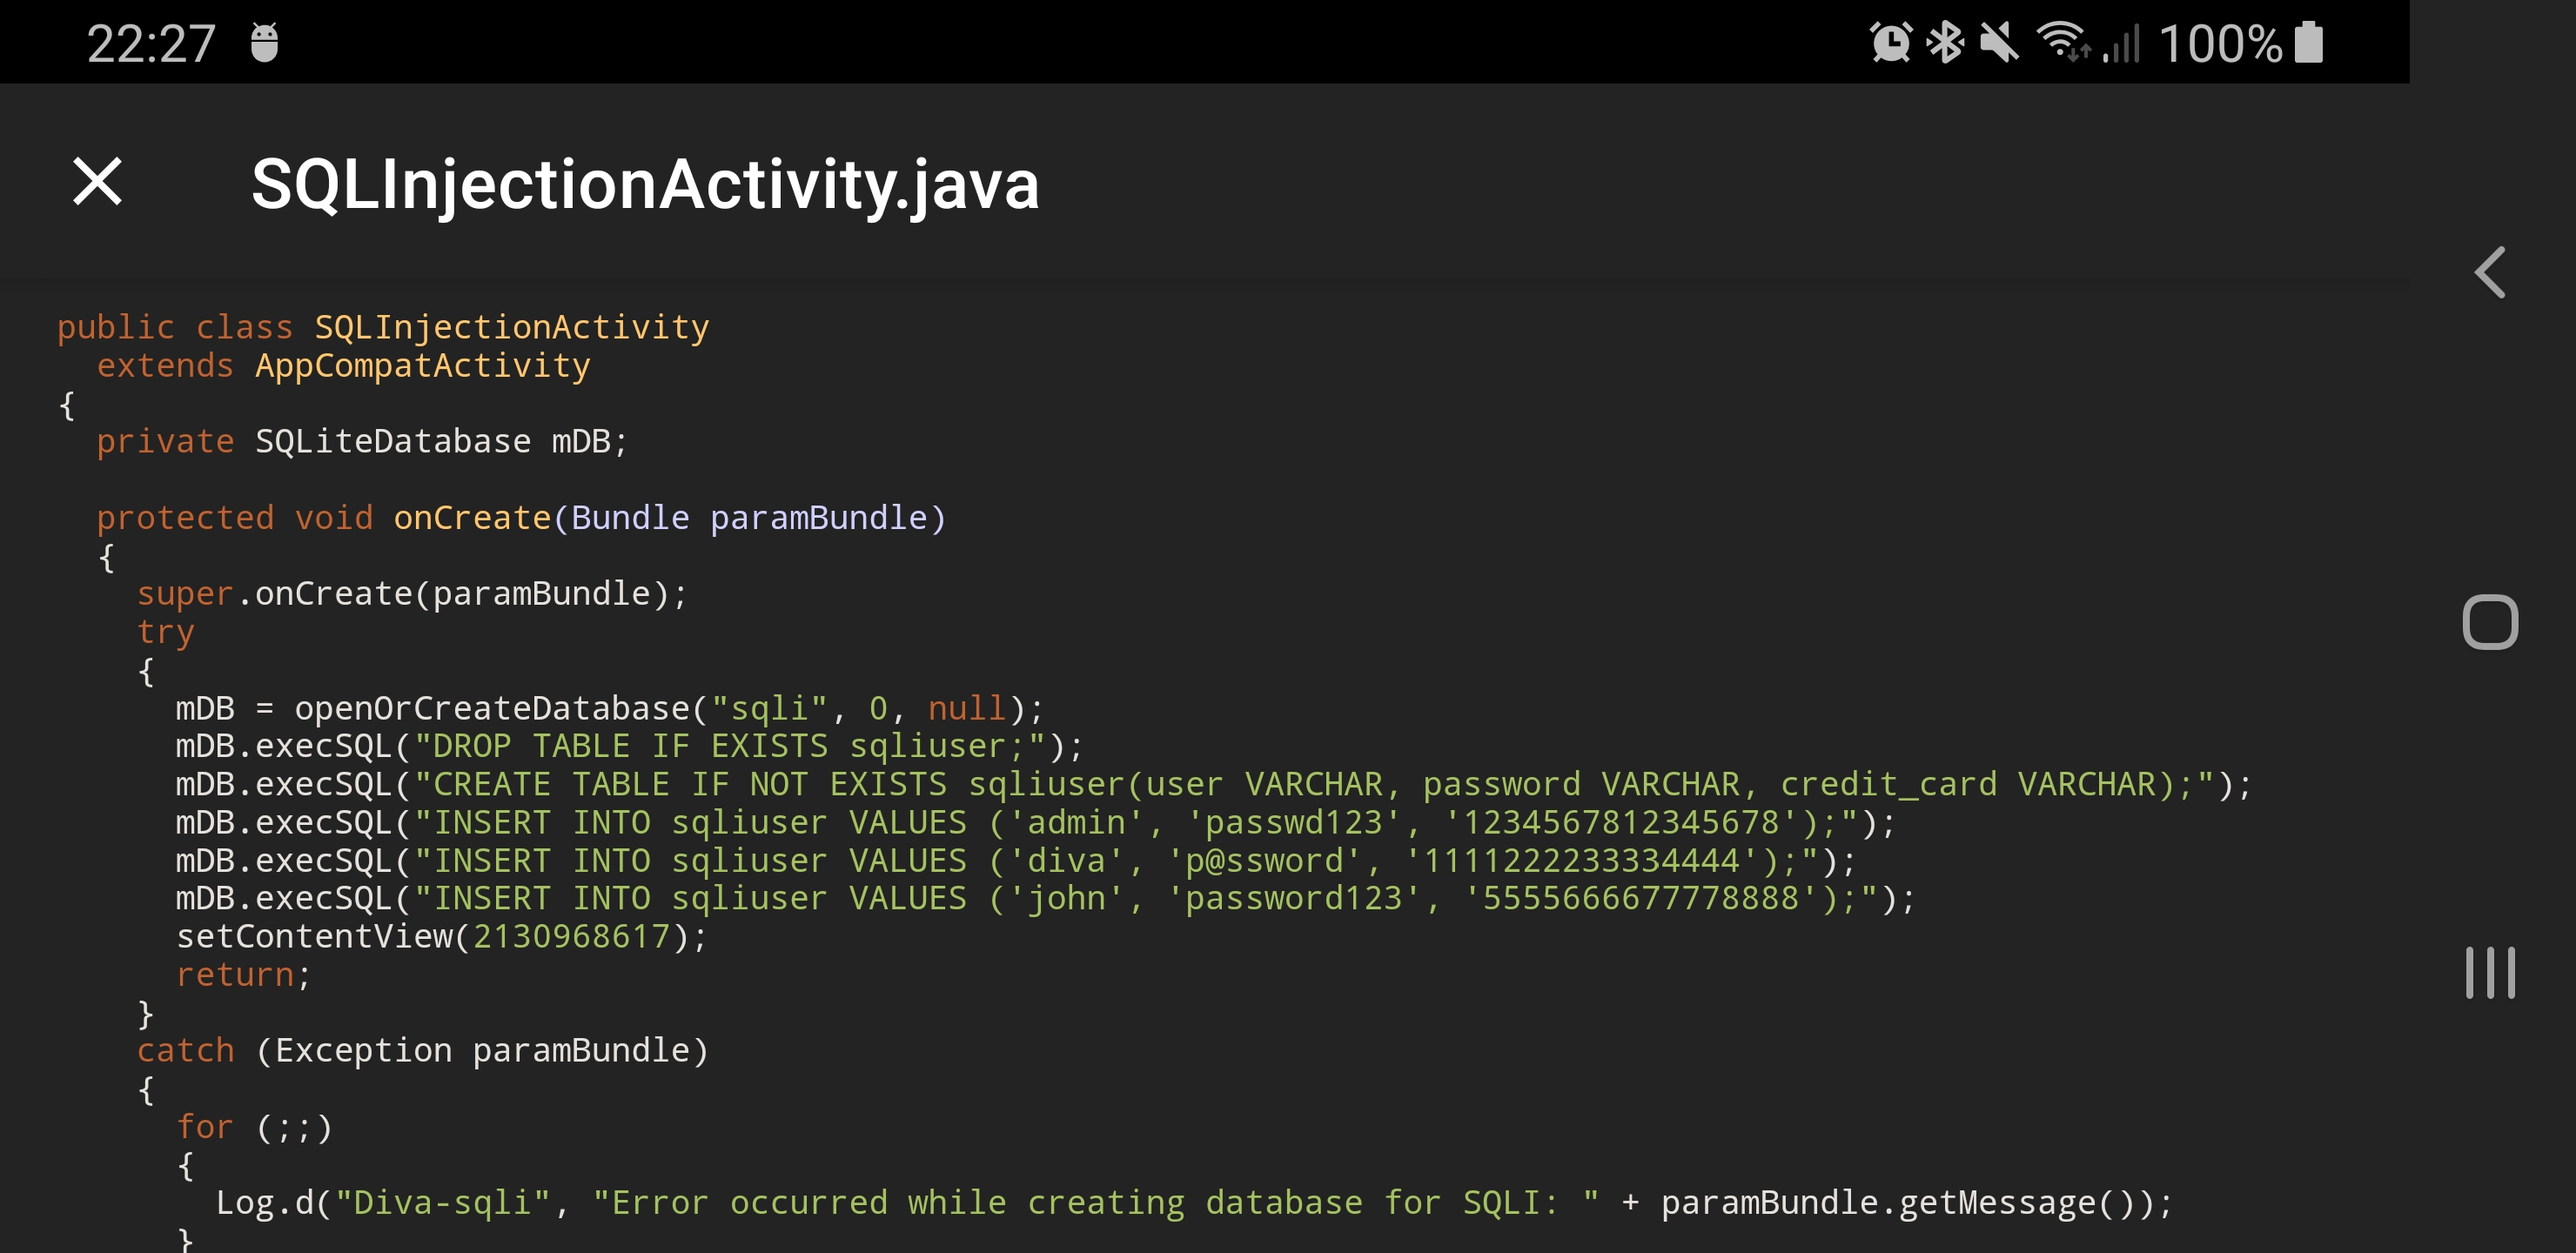
\includegraphics[width=15cm]{pictures/codeview}
	\caption{A visszafejtett forráskód megjelenítése szintaktikai kijelöléssel.}
	\label{codeview}
\end{figure}

\newpage

\subsection{Espresso}

Az Android Studio rendelkezik jó pár funkcióval, amikről már tettem említést.
Amit szándékosan kihagytam, az a UI\footnote{User Interface} tesztek felvétele.
Az Espresso Test Recorder funkció által megtehetjük, hogy nem kézzel írjuk a teszteket, hanem felvesszük őket.
Feltudjuk venni az interakcióinkat az alkalmazással és ellenőrizni tudjuk az elemeket a felhasználói felületen, valamint biztosítani tudjuk az adott pillant kép helyességét.
Az Espresso Test Recorder veszi az elmentett teszt felvételt és automatikusan generál egy hozzátartozó UI tesztet, amit aztán futtatni tudunk az alkalmazásunk tesztelése érdekében.

Espresso Test Recorder az Espresso Testing keretrendszer alapján írja a teszteket, ami egy API az AndroidX Test-ben.
Segít megbízható és tömör UI teszteket írni a felhasználói interakcióra alapozva.
Állíthatunk elvárásokat és interakciókat anélkül, hogy hozzáférnénk az alkalmazás nézeteihez és activity-jeihez.
Ez a struktúra optimizálja a tesztek futási idejét. \cite{espresso}

A projektem esetében nem volt ilyen egyszerű a helyzet.
Mindenképpen segített, hogy feltudtam venni a teszteket, de vegyük a következő helyzetet.
Tegyünk fel, hogy a bejelentkezés folyamatára már készen van a teszt.
Amikor Espresso-val tesztet veszünk fel, az alkalmazás tiszta állapotról indul.
Ez az jelenti, hogy ha bármilyen bejelentkezés utáni interakciót szeretnénk felvenni, akkor a teszt a bejelentkezéssel együtt kezdődik.
Az ilyen problémákat manuálisan kell kikerülni.
A \ref{espressotest} kódrészletben megfigyelhető, hogy egy \emph{@Before} annotációval ellátott metódusban elmentettem egy teszt felhasználó nevet és jelszót.
Ezután pedig egyszerűen egy Intent segítségével elindítottam az Activity-t.
Mindez nem volt elegendő ahhoz, hogy sikeresen tovább mehessek ugyanis bejelentkezés után történik a különböző engedélyek ellenőrzése.
Az Espresso arra is nyújt megoldást, hogy ezeket az engedély kéréseket automatikusan elfogadjuk a tesztekben a \emph{GrantPermissionRule} osztály segítségével.

\inputminted[linenos=true, breaklines]{java}{./codes/test.java}
\captionof{listing}{Espresso UI teszt az adatok törléséhez.\label{espressotest}}

\subsection{Material Design 2.0}

Az alkalmazás elkészítésekor próbáltam figyelembe venni a felhasználói interfésszel kapcsolatban támasztott ki nem mondott elvárásokat.
Korábbi Play Store-ban publikált alkalmazásaim alapján mondhatom, hogy a felhasználónak az app megjelenése legalább olyan fontos, mint a funkcionalitása.
A Google már korábban, az Android 5.0 (API verzió 21) verzióval hozta be az akkoriban még újnak számító Material Design-t és teljesen megreformálta az Android platform felületét.
Sok embernek tetszettek az élénk színek és a vetett árnyákok, amik meghatározó részei voltak a komponenseknek. Persze, ez nem volt tökéletes.
A nevéből is ered, hogy az anyagokból kiindulva és azok egymásra pakolásával született meg a dizájn. 
Kicsit pontosabban fogalmazva a Material Design irányelveket foglal össze, amiket nem fontos követni, de ajánlott. 
A Material Design 2 nem hozott hatalmas eltéréseket elődjéhez képest, inkább csak letisztultabb lett, ami szimplán jobb vizuális élményt nyújt.
Az Android platformot tekintve új komponensek érkeztek, ezek közé tartozik a \emph{BottomAppBar} és a \emph{Chip}.

% https://material.io/develop/android/docs/getting-started/

\chapter{A visszafejtés teszteléséhez felhasznált programok}\label{teszteles}

\section{Sérülékeny Android alkalmazások}

A teszteléshez keresnem kellett olyan sérülékeny alkalmazásokat, amelyeken jól lehet demonstrálni a visszafejtést.
Minden alkalmazás, amit itt megemlítek nyílt forráskódú és kimondottan erre a célra készítették őket.
Ez azért is jó, mert a visszafejtett kódot össze lehet hasonlítani az eredetivel és megnézni mennyire volt hatékony a visszafejtési folyamat.
A jogi következményei egy ilyen visszafejtésnek elég ködösek.
Szerettem volna biztosra menni, ezért is választottam nyílt forráskódú, szabadon elérhető alkalmazásokat teszteléshez, mert így érezhetem magam a legnagyobb biztonságban.
A következő lista tartalmazza a teszteléshez felhasznált szándékosan sérülékeny alkalmazásokat.

\begin{enumerate}
	\item
	\begin{description}
		\item[Damn Insecure and Vulnerable Application (Diva)] Talán kicsit régi, mert több mint 3 éve nem volt frissítve. Ettől függetlenül ezzel értem el a legjobb eredményt és ezt találtam a leghasznosabbnak.\newline  Megtalálható itt: \url{https://github.com/payatu/diva-android}.
	\end{description}
	\item
	\begin{description}
		\item [Frida] Ez egy általam fejlesztett alkalmazás, ami kimondottam dinamikus intrumentáció tesztelésére és bemutatására készült.\newline Megtalálható itt: \url{https://github.com/t0thkr1s/frida-demo}
	\end{description}
	\item
	\begin{description}
		\item [Purposefully Insecure and Vulnerable Android Application(Pivaa)] A Pivaa egy kicsit modernebb verziója a Diva alkamzasának. Rendkívül sok sérülékenységet tartalmaz, amiből sokat lehet tanulni.\newline Megtalálható itt: \url{https://github.com/HTBridge/pivaa}
	\end{description}
\end{enumerate}

A többi alkalmazást a \url{https://github.com/as0ler/Android-Examples} repository-ból használtam fel, ami nem csak applikációkat tartalmaz, hanem játékokat is.
A forráskód itt nem érhető el, viszont visszafejtés után betekintést nyerhetünk játékok felépítésébe is.

\chapter{Megvalósított funkciók}\label{funkciok}

\section{Regisztráció}

A szolgáltatást nem akartam mindenki számára elérhetővé tenni, csak a regisztrált felhasználóknak.
A \ref{registration} ábrán látható a regisztrációs felület.
Igazából semmi különösebb mezőt nem tartalmaz, csak a szokásos adatokat kell megadnia annak, aki igénybe szeretné venni a szolgáltatást.
Ha a regisztráció sikeresen befejeződött, akkor vissza irányítom a felhasználót a bejelentkezési felületre.
A folyamatot próbáltam minél egyszerűbbre és magától értetődőre tervezni.

A mezőket tekintve \emph{TextInputLayout}-ba ágyazott \emph{TextInputEditText}-et használtam.
A \emph{TextInputLayout} rendelkezik, olyan tulajdonságokkal, mint például a segítséget nyújtó szöveg és az animáció.
Ez által még nyilvánvalóbb, hogy melyik mezőbe mit kell írni.

Számításba vettem, hogy a felhasználó nem biztos, hogy álló helyzetben fogja tartani a telefonját, ezért külön layout fájlokat készítettem a fekvő nézethez.
Szerencsére nem kellet minden felülethez külön fekvő nézetet késztenem, csak a regisztrációhoz és a bejelentkezéshez.

\section{Bejelentkezés}

Természetesen regisztrálás után a felhasználónak be kell jelentkeznie, hogy hozzáférhessen azokhoz a végpontokhoz, amik bejelentkezéshez vannak kötve.
Lényegében az összes lényeges végpont bejelentkezéshez van kötve, ezért mondhatjuk, hogy a bejelentkezést kötelező megtenni.

A felület itt csak két mezőt tartalmaz, a felhasználó nevet és a jelszót.
Mivel ez egy folyamatban lévő fejlesztés nem tartottam prioritásnak a jelszó visszaállítás funkció implementálását, ebben a korai verzióban.
A jelszó mezőben bekapcsoltam egy úgynevezett jelszó kapcsolót, ami a mező jobb szélén látható.
Segítségével a felhasználók láthatóvá tehetik a beírt jelszójukat és ellenőrizhetik annak helyességét.

Alapvetően a \emph{MainActivity} indul az alkalmazás futtatásakor és az \emph{AuthenticationActivity} csak akkor indul, ha nincsen mentett felhasználónév és jelszó páros.
Az \emph{AuthenticationActivity} tartalmazza mind a bejelentkezési, mind a regisztrációs fragment komponenst.

\begin{figure}[!h]
	\centering
	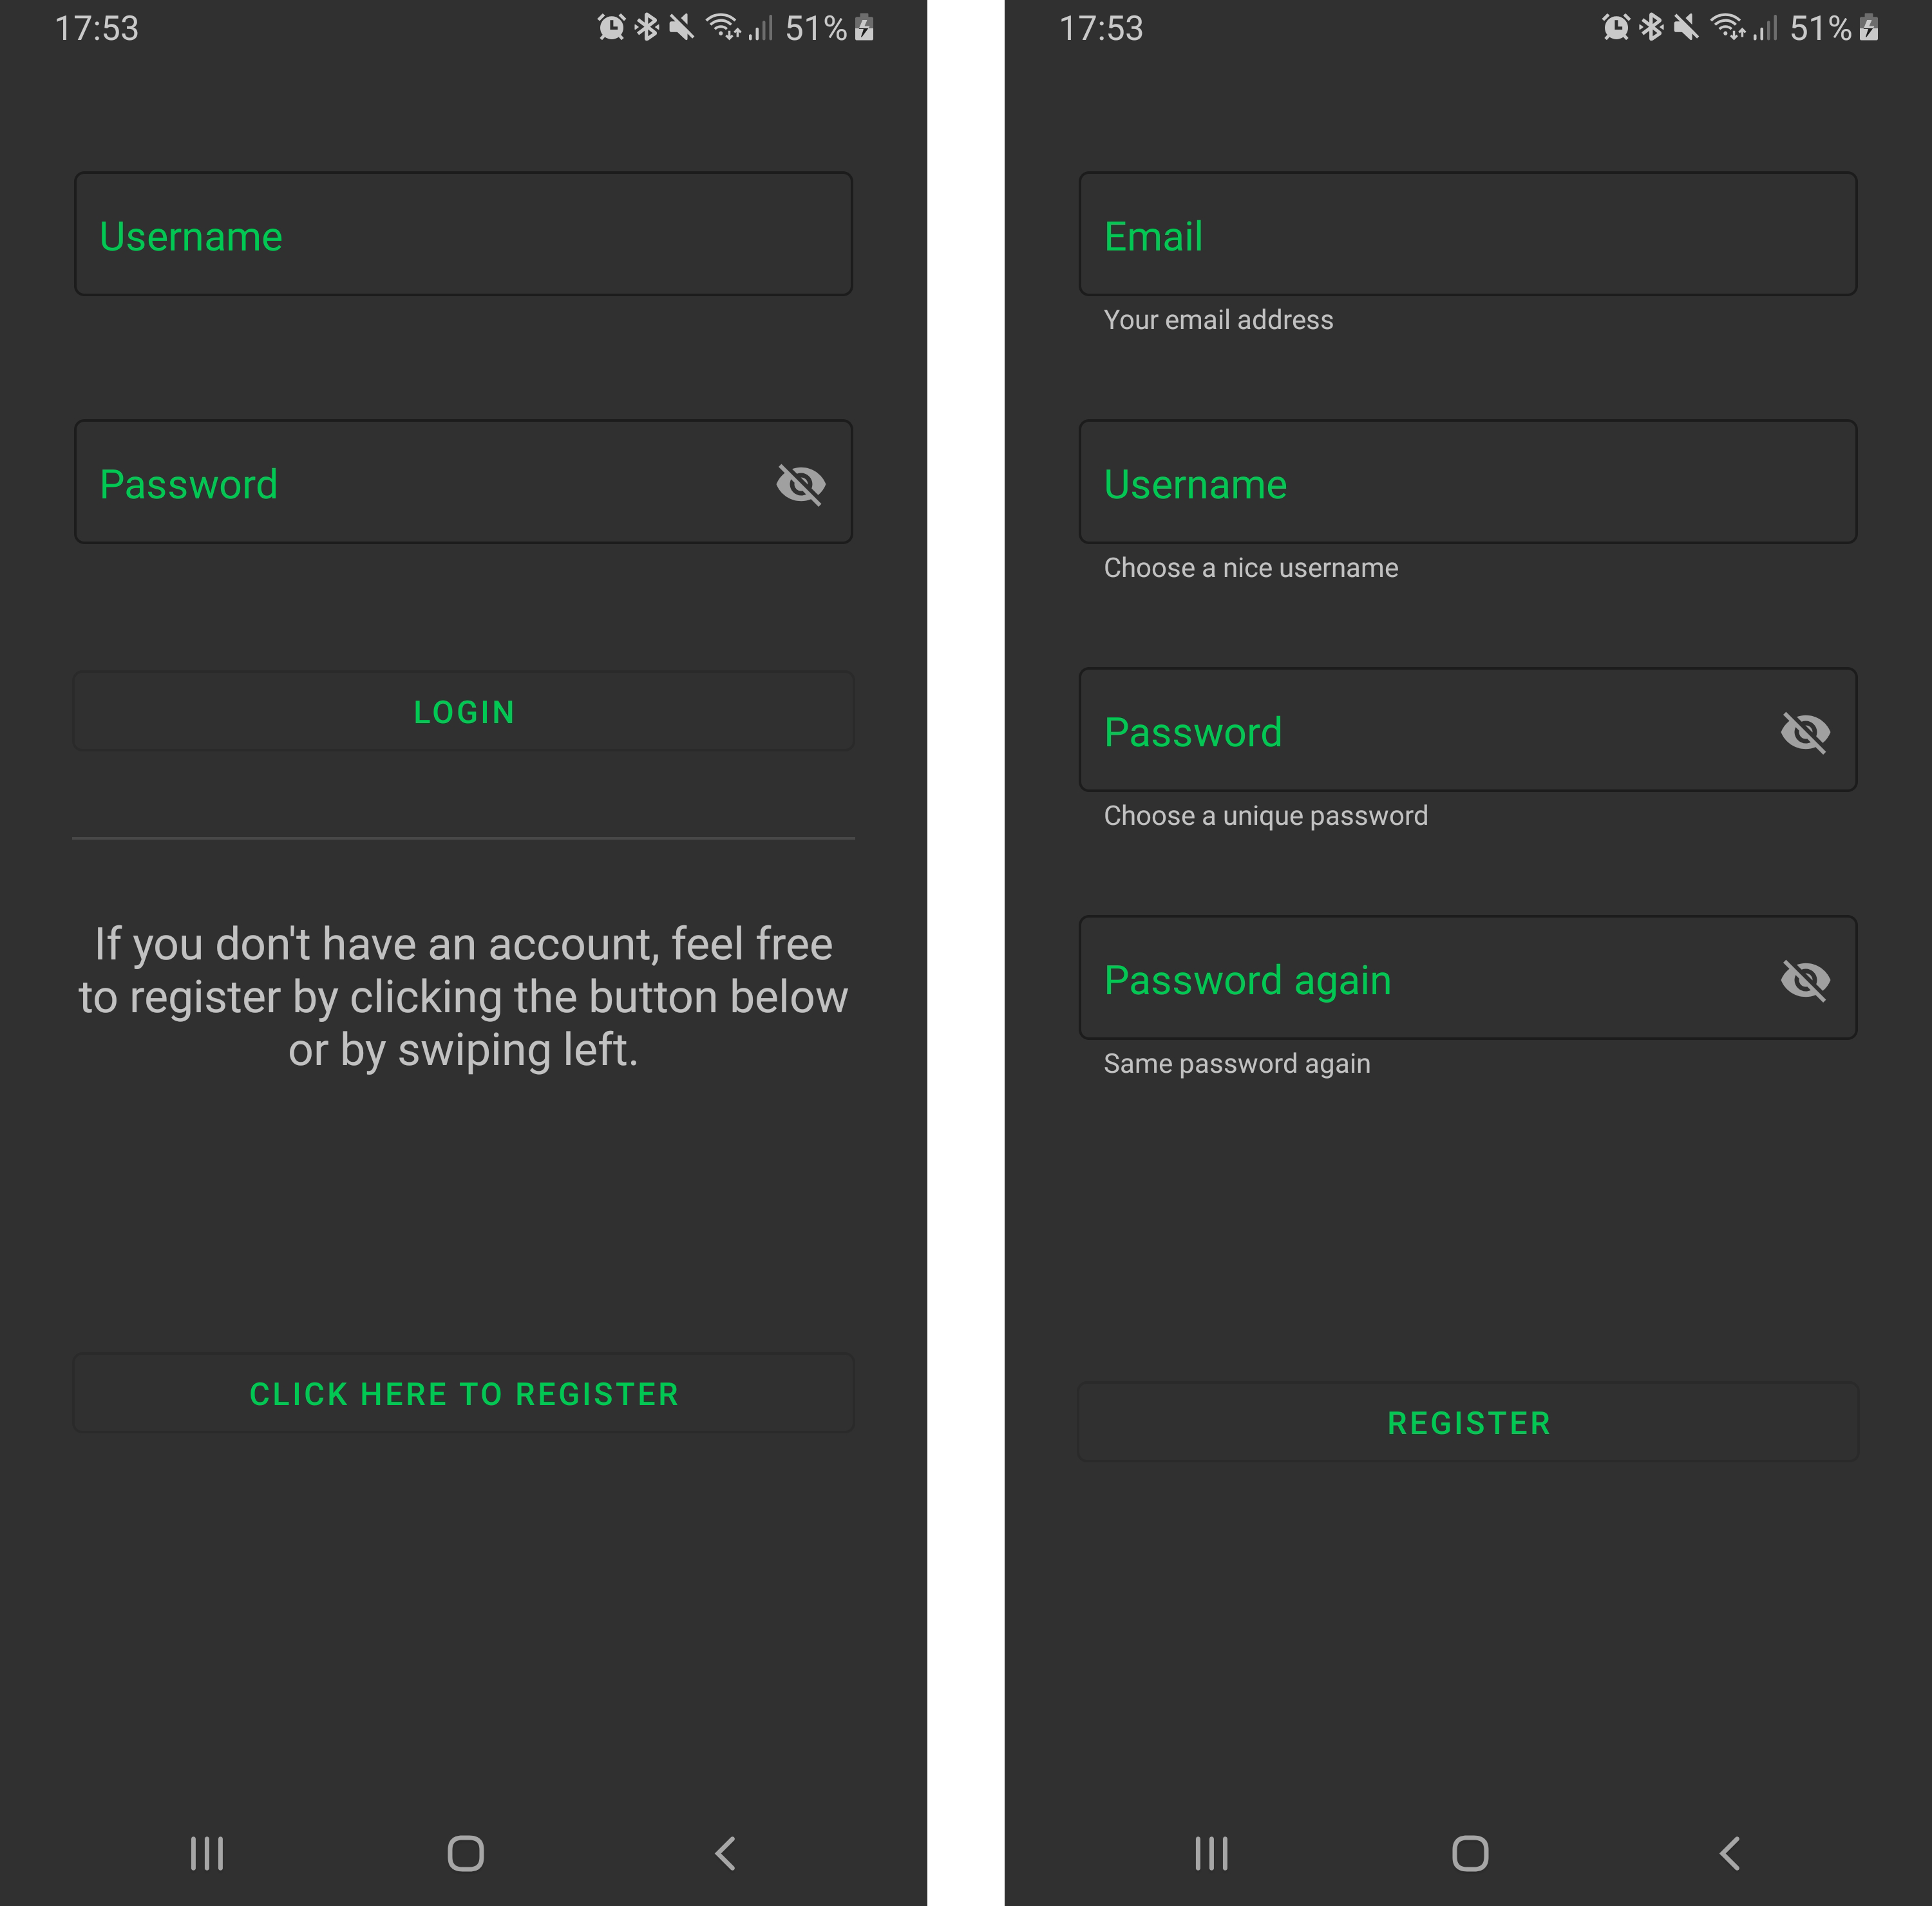
\includegraphics[height=15cm]{pictures/android_login_registration}
	\caption{A bejelentkezési és regisztrációs felület megvalósítása.}
	\label{registration}
\end{figure}

\section{Kijelentkezés}

Szerver oldalon csak az \emph{Authorization Header} van ellenőrizve, ami azt jelenti, hogy minden egyes hálózati kérésben benne kell hogy legyen.
Ennek a kezelését úgy oldottam meg, hogy sikeres bejentkezés után \emph{SharedPreferences} használatával eltároltam a felhasználónevet és a jelszót.
Amíg nem történik kijelentkezés, addig ezek az adatok mentve maradnak.

A \ref{saving_sharedpref} kódrészleten láthatjuk, hogyan történik az adatok mentése.
A \emph{SharedPreferences} segítségével kulcs-érték párokat tárolhatunk biztonségos módon.
A \emph{getSharedPreferences()} metódus 2 paramétert vár, az egyik a név, a másik a használni kívánt mód. 
Névnek az alkalmazás csomag nevét választottam és privát módban hoztam létre, hogy csak az én alkalmazásom férhessen hozzá az adatokhoz.

\begin{listing}[ht]
	\inputminted[linenos=true, breaklines]{java}{./codes/saving_sharedpref.java}
	\caption{Adatok mentése \emph{SharedPreferences} segítségével.}
	\label{saving_sharedpref}
\end{listing}

% \lstinputlisting[language=Java, label={saving_sharedpref}, caption=]{./codes/saving_sharedpref.java}

A \ref{deleting_sharedpref} kódrészletben láthatód metódus nem sok eltérést mutat, viszont elengedhetetlen volt ahhoz, hogy töröljem az összes \emph{SharedPreferences}-be mentett adatot.

\begin{listing}[ht]
	\inputminted[linenos=true, breaklines]{java}{./codes/deleting_sharedprefs.java}
	\caption{Az összes \emph{SharedPreferences}-be mentett adat törlése.}
	\label{deleting_sharedpref}
\end{listing}

% \lstinputlisting[language=Java, label={deleting_sharedpref}, caption=Az összes \emph{SharedPreferences}-be mentett adat törlése.]{./codes/deleting_sharedprefs.java}

\section{Adatok törlése}

A kliens oldalon elég sok adat jelenik meg, ami természetesen tárolva van.
Ilyen például a feltöltések listája, értesítések és a letöltött fájlok is ide tartoznak.
Az adatok törlése funkcióval biztosítottam, hogy a felhasználónak lehetősége legyen törölni minden adatot és előzményt.
Ide tartozik a gyorsítótárba másolt feltöltött alkalmazások, amik egy idő után értékes tárhelyet foglalhatnak el.
Nem beszélve arról, hogy az adatbázisban lévő összes tábla adatát ürítem.
Lehetséges, hogy kényelmesebb lett volna, ha a felhasználó maga választja ki mit szeretne törölni.
Sajnos ez a korai verzió csak az együttes törlést biztosítja.
Jól jöhet ez a funkció akkor is ha a telefon esetleg nem rendelkezik elég tárhellyel vagy egyszerűen csak helyet szeretnénk felszabadítani.

\section{Fájl feltöltés}

Az alkalmazás egy alapvető funkciója, hogy fel tudjuk tölteni az APK fájlokat.
Ezt a funkciót próbáltam a legkézenfekvőbb helyen elhelyezni, mert ezzel indul az egész folyamat és magától értetődőnek kell lennie.
Ezért lett a legeleső fragment a feltöltések listáját tartalmazó fragment.
Ebben a feltöltési listában jelenítem meg a feltöltött APK fájlok neveit és a feltöltés dátumát.

A feltöltéshez a felhasználónak egy jól látható \emph{FloatingActionButton} komponensre kell kattintania.
A tervezési szakaszban úgy gondoltam, hogy hasznos lenne egy saját fájl kiválasztó felületet készíteni.
Aztán hamar rájöttem, hogy teljesen felesleges újra feltalálni a spanyol viaszt és nem kellene haszontalan felületekkel bonyolítani az applikációt.
Biztos találkoztunk már olyan alkalmazással, ami elindított egy külső alkalmazást csak hogy elvégezzel valamilyen feladatot.
Én is egy ilyen megoldást alkalmaztam.
Nem csak \emph{Activity}-ket tudunk indítani \emph{Intent}-ek segítségével, hanem különböző műveleteket is elvégezhetünk.
Az ilyen \emph{Intent}-eket \emph{Implicit Intent}-eknek nevezzük.
Példának okáért, a fájl kiválasztás egy ilyen művelet.
\emph{Implicit intent} használatával indítottam el a fájl kiválasztást, aminek többek között megadtam, hogy milyen típusú fájlokat szeretnék kiválasztani.
Ez a típus természetesen a \emph{application/vnd.android.package-archive} volt, ami megfelel az Android telepítő fájloknak.
Ebben az esetben nincs lehetőségünk más típusú fájlt kiválasztani csak a megadottat.

A fájl kivlasztása után az \emph{onActivityResult} metódus \emph{Intent} típusú paraméterében kapjuk meg az URI\footnote{Uniform Resource Identifier}-t.
Ezt az URI-t felhasználva elmentettem a fájlt az alkalmazás gyorsítótárába.
Erre azért volt szükség, mert különben nem kaptam volna meg az abszolút elérési útvonalat.
Eztán már csak service elindítása maradt hátra. 

A \emph{startService(Intent service)} metódus egy \emph{Intent}-et vár, ami segítségével elindíthatjuk a háttér service-t.
Fontos, hogy ez még így nem elég, hanem extraként hozzá kell adni a feltölteni kívánt fájlt.
A \ref{uploads_notifications} ábra bal oldali képernyőképén látható a feltöltött fájlok listája.

\section{Fájl letöltés}

A fájl letöltés is egy roppant fontos funkció, ugyanis csak így jut el a felhasználóhoz az elkészült projekt.
A megvalósítását hozzákötöttem az értesítésekhez, mert a kliens abban kapja vissza a letöltendő fájl nevét.
Megfigyelhetjük a \ref{uploads_notifications} ábra jobb oldali képernyőképén, hogy minden egyes értesítés kártyáján ott a letöltés gomb.
Ha ezekre rákattintunk, akkor itt is minden egyes alkalommal egy újabb háttér service fog elindulni.
Azt is megtehetjük, hogy akár többször is letöltjük ugyanazt a fájlt.
Ha már lokálisan létezik egy ugyanolyan nevű projekt, mint amit éppen letöltünk akkor sem kell félnünk, hogy felül írjuk, mert egyedi nevet fog kapni.
Ezt úgy valósítottam meg, hogy ha létezik már a projekt mappája, akkor hozzáfőzök egy számot és 0-tól kezdődően mindig növelem.

\begin{figure}[!h]
	\centering
	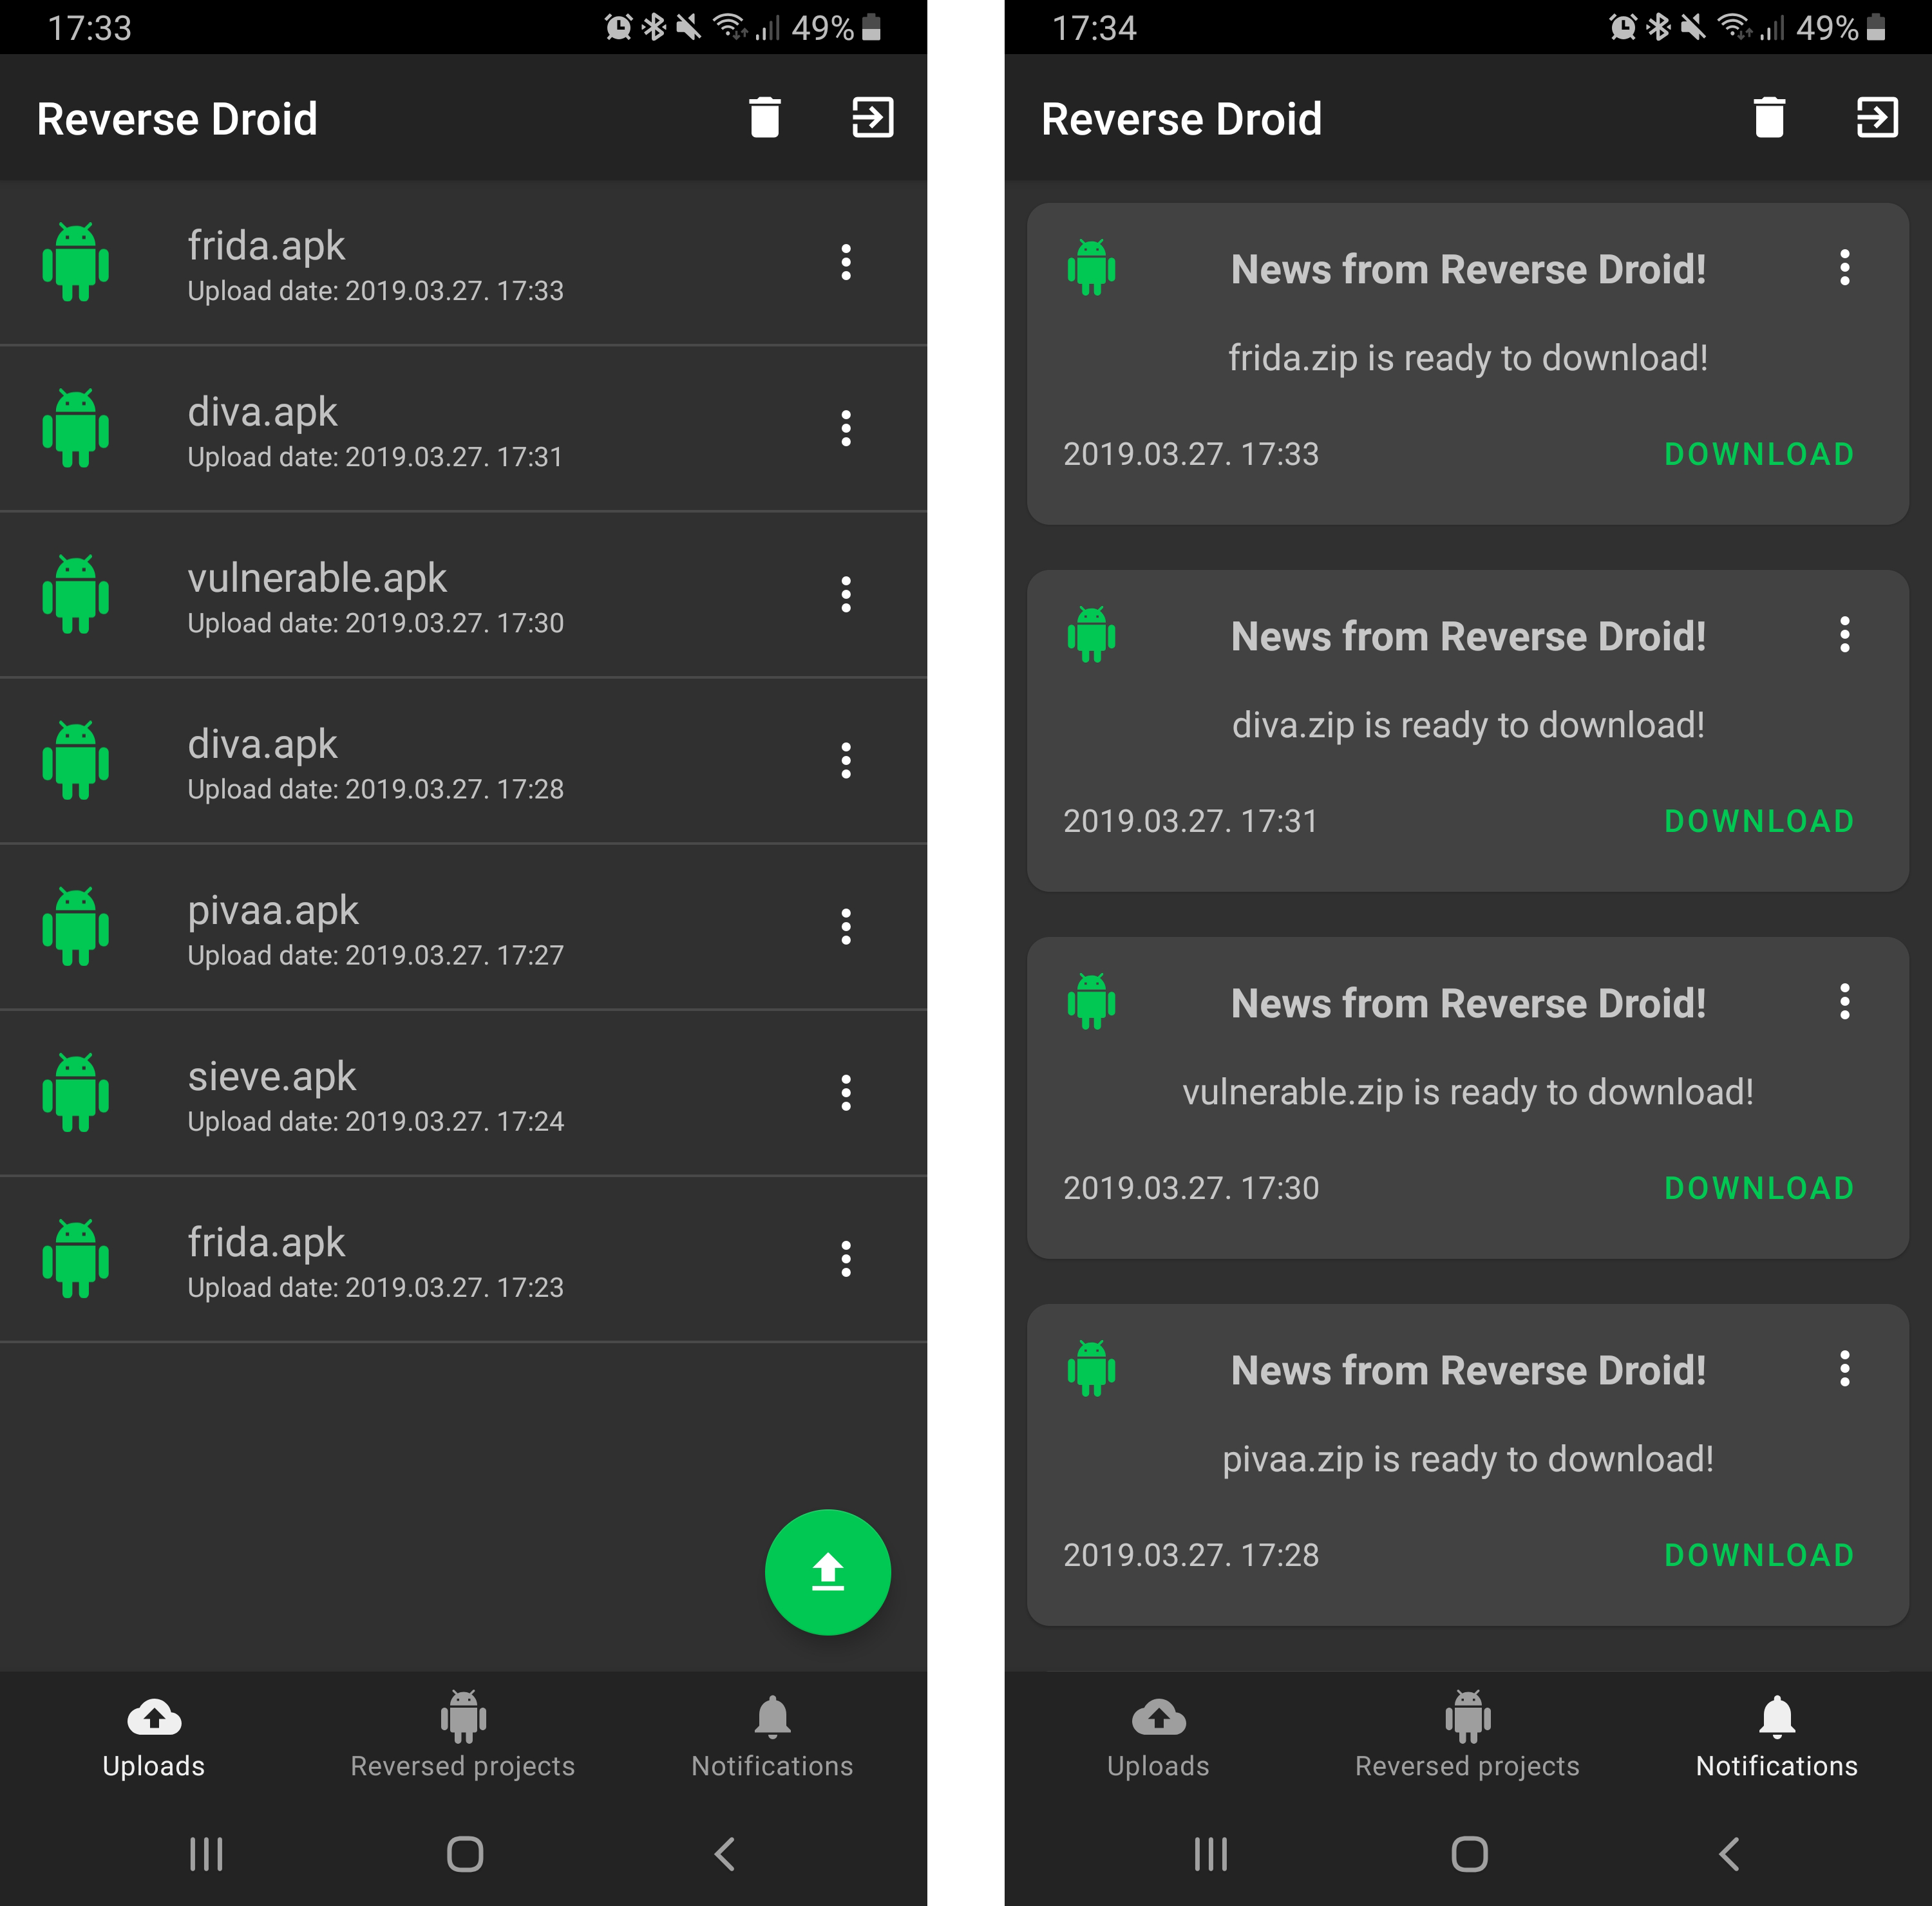
\includegraphics[height=15cm]{pictures/android_uploads_notifications}
	\caption{A feltöltött APK fájlok és értesítések felülete.}
	\label{uploads_notifications}
\end{figure}

\section{Navigáció a fájlrendszerben}

A letöltött és kitömörített projektek az alkalmazás mappájában kerülnek.
Ennek a mappának a neve megegyezik az alkalmazás nevével és az elsődleges külső tárhelyen foglal helyet.
Ezzel alapvetően nincs is semmi probléma, csak ha megszeretnénk nézni a fájlokat, akkor el kellene hagynunk az alkalmazást.
Ez pedig rossz felhasználói élményhez vezetett volna.
Ennek megoldására megvalósítottam egy nagyon egyszerű fájl rendszer navigációt, de ezt csak az alkalmazás mappájában tettem lehetővé.
Szóval a felhasználó nem tud a fájlrendszerben feljebb navigálni, csak a ,,Reverse Droid'' gyökér mappáig.
Ezzel a funkcióval kitömörítés után egyszerűen és gyorsan elérhetővé válik a projekt a felhasználó számára.
A mappák esetében megjelenítettem a módosítás dátumát és hogy hány fájlt/mappát tartlmaz.
A fájlok részleteit tekintve a fájl nevét, módosítás dátumát és a fájl méretét is megjelenítettem.

Ezeken felül hozzáadtam egy olyan funkciót, hogy ha hosszan kattintunk egy mappán, akkor lehetőséget kapunk annak törlésére.
Ha nem egy mappán kattintunk hosszan, hanem egy fájlon, akkor három opció közül is választhatunk.
Az első triviális funkció itt is a fájl törlése volt, a második a fájl megosztása kompatibilis külső alkalmazással.
Végül, de nem utolsó sorban a kód megtekintése menü pont kapott helyet.
Ennek a működéséről és megvalósításáról már említést tettem a \nameref{code_view} alfejezetben, de nem említettem meg minden részletet.
Kimaradt példul az, hogy csak bizonyos fájlkiterjesztéseket támogatok jelen helyzetben.
Mivel a forráskód tartalmazza az igazán érdekes dolgokat, ezért arra koncetráltam, hogy legalább az Android projektekre jellemző szöveges fájlkiterjesztéseket támogassam.
A különböző képek és speciális fájlok megjelenítése egyenlőre nincsen támogatva, de ez is egy olyan funkció, amit megszeretnék valósítani a jövőre nézve.
A támogatott kiterjesztéseket jelenleg az is befolyásolja, hogy maga a \emph{CodeView} miket támogat.

A visszalépés megvalósítása okozott egy kisebb fejtörést.
A vissza gomb megnyomására túlságosan is bonyodalmas lett volna megvalóstani a visszalépést, ezért úgy döntöttem, hogy egy külön elemmel fogom ezt kivitelezni.
Ez az elem úgymond egy speciális lista elem, amit akkor jelenítek meg ha nem az alkalmazás mappájában tartózkodunk.
Emlékeim szerint több fájl kezelő is használta már ezt a megoldást és elég hatékonynak tűnt ez a fajta visszalépési technika.

\section{Értesítések}\label{ertesitesek}

Az értesítések küldése és fogadása szintén egy kulcs fontosságú része az alkalmazásnak, ezt már többször is hangsúlyoztam.
A fájlok letöltése és kitömörítése mérettől, valamint hálózati kapcsolattól függően időt vesz igénybe.
Az elején úgy gondoltam, hogy egy egyszerű \emph{Toast} üzenet is elég a feltöltés állapotának visszajelzésére.
Aztán hamar rákellett jönnöm, hogy ez nem ad elég információt a felhasználó számára, ráadásul rossz felhasználói élményhez is vezet.
Végül úgy döntöttem, hogy feltöltést is hasonlóan valósítom meg, mint a letöltést.

A \ref{notifications} ábrán láthatóak az alkalmazásban használt értesítések.
Ez a három értesítés jól érzékelteti a három fő funkcióját az applikációnak.
Ezeket össze is foglaltam a következő listában:

\begin{enumerate}
	\item Android telepítő fájl feltöltése
	\item Értesítés a projekt készenlétéről
	\item Az elkészült tömörített projekt letöltése
\end{enumerate}

A megvalósítást illetően az első és a harmadik funkció megvalósítása kliens oldalon történt teljes egészében.
A harmadik természetesen a szerverről érkezik, ha befejeződött a fájl feldolgozása.
Ezek mind az adott körülményektől függnek, ezért azzal is számolni kell, hogy jelentős időtartamot igényelnek.
Azt is lehetővé szerettem volna tenni a felhasználó részére, hogy a műveletek között is elhagyhassa az applikációt.

Itt is a háttér service volt az az applikáció komponens, amit ennek kivitelezésére felhasználtam.
Segítségével hosszabb ideig tartó műveleteket tudunk végezni, anélkül hogy a felhasználó interakcióba lépnek az applikációval.

\begin{figure}[!h]
	\centering
	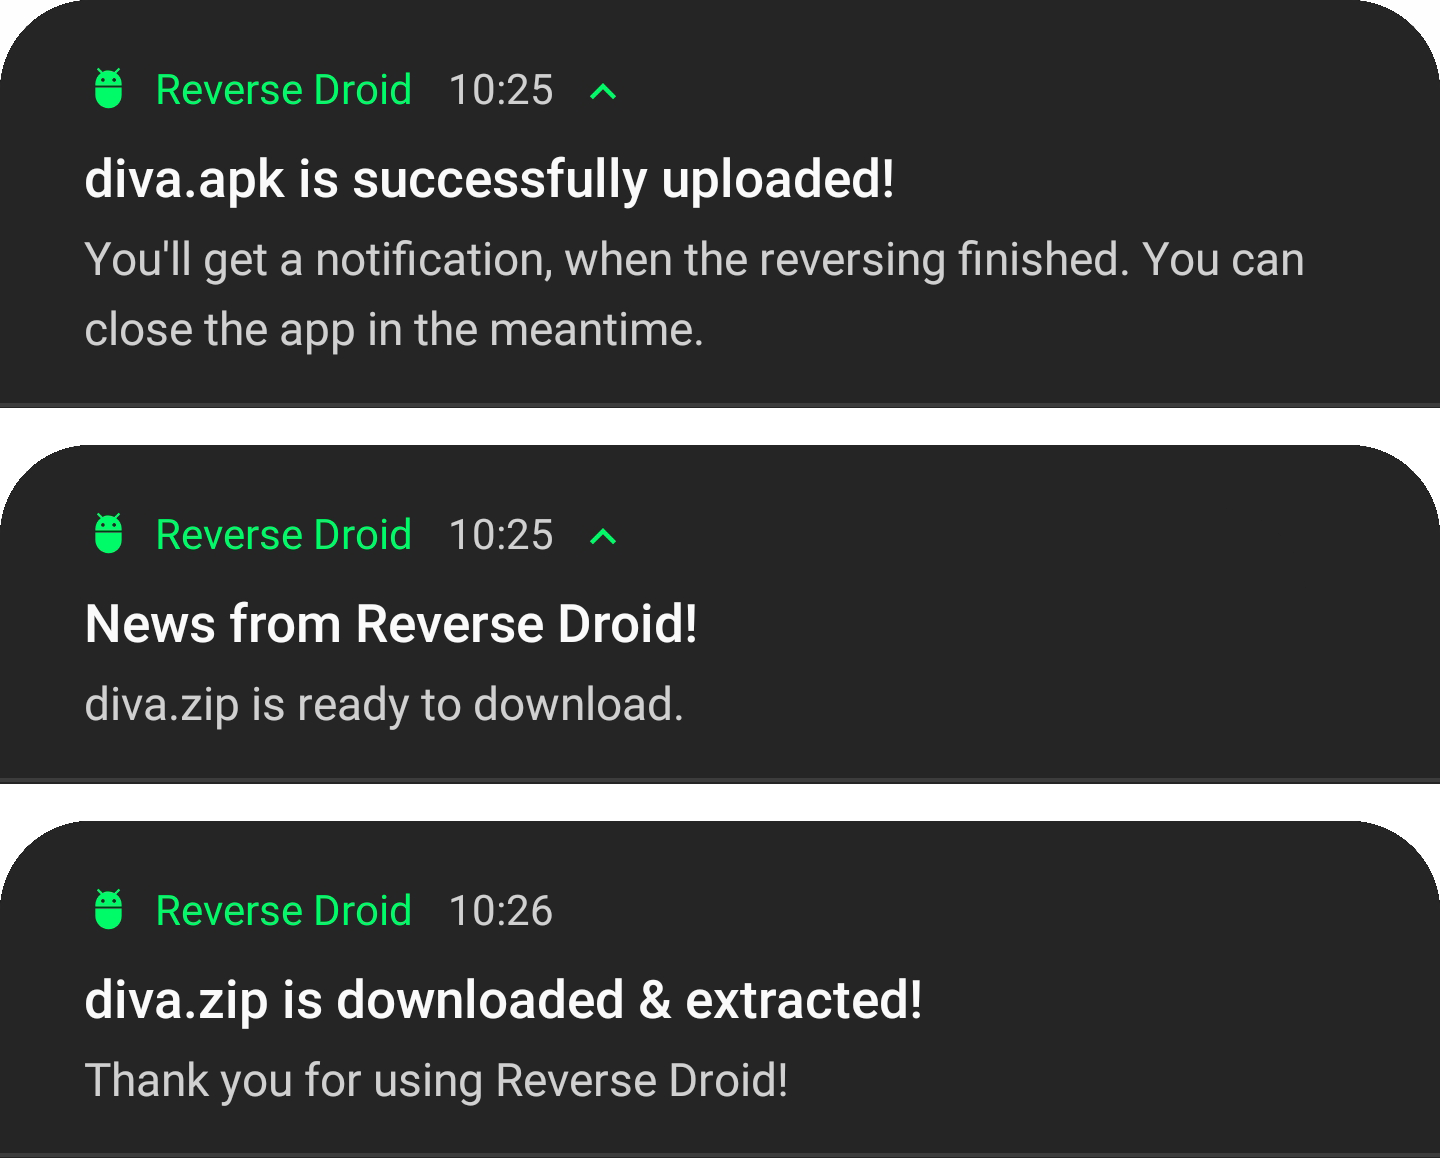
\includegraphics[height=10cm]{pictures/notifications}
	\caption{Az alkalmazásban megjelenő értesítések.}
	\label{notifications}
\end{figure}

\chapter{Továbbfejlesztési lehetőségek}\label{lehetosegek}

Úgy gondolom, hogy sokkal nagyobb piaci érték rejlik ebben az alkalmazásban, mint amennyit egyedül sikerült megvalósítanom.
A jövőben is szeretném folytatni a fejlesztést és esetlegesen nyílt forráskódúvá tenni a projekteket, hogy mások is közre tudjanak működni a fejlesztésben.

Szeretnék több figyelmet fordítani a biztonságra és hatékonyságra. 
Gondolok itt a biztonságos kommunikációra TLS-es keresztül és a harmadik féltől származó könyvtárak csökkentésére.
Azért lenne érdemes minimalizálni a harmadik féltől származó könyvtárakat, mert nem mindig tudjuk milyen kódot tartalmaznak és mennyire tartják karban a kód bázist.

Jelenleg csak a forráskódok megjelentését támogatja az alkalmazás, de jó lenne ha különböző fájl típusokat is megtudna jeleníteni.
Például a képek vagy adatbázisok megtekintése is kritikus lehet egy Android alkalmazás elemzésekor.
A kód visszafejtése végén egy összegző report is hasznos lehetne a felhasználó számára, ami tartalmazná a feldolgozott fájlok számát és egy gyors áttekintést nyújtana az adott alkalmazással kapcsolatban.

Egy forráskód elemző integrálása is jelentős előnnyel járhat a többi alkalmazással szemben. Hasonlóan a Google Play Protect-hez, jelezhetnénk a felhasználó számára, ha a feltöltött \emph{apk} malware.
Találkoztam több webes \emph{apk} analizálóval, ahol csak az Android komponenseket emelték ki, de az elemzést már a felhasználóra bízták.
Nyilván nem lenne célszerű mindent egy algoritmusra bízni, de mindenesetre könnyebbséget látok egy átfogó analízisben, ami esetlegesen mestersége intelligenciára alapul.

\chapter{Tapasztalatok}\label{tapasztalatok}

Úgy érzem elértem a célom ezzel a projekttel és sokat sikerült tanulnom az elkészítése alatt.
Új technológiákat ismertem meg és használtam. Nem állítom, hogy hibamentes és minden működik, hiszen ez mégis csak egy szoftver, amit folyamatosan karban kell tartani és fejleszteni.
A fejlesztés minden fázisában találtam valami kihívást, ami segítette a fejlődésemet és arra ösztönzött, hogy jobban megismerjem az adott technológiát.

Természetesen nem volt minden magától értetődő és jó pár nehézséggel is találkoztam, amiket már korábban meg is említettem.
Számomra, ha valami nem sikerült az mindig ösztönzőleg hatott és motivált a tanulásban. Sikerült az idegen technológiák iránt érzett kíváncsiságom is kielégíteni.
A reverse engineering világába is betekintést nyertem, ami különösen érdekelt engem. 

A fejlesztésnél csak egyetlen kellemetlen dologgal találkoztam. Szerintem sok fejlesztő egyet ért ha azt mondom, hogy a hiányos vagy éppen félre vezető dokumentáció a legnagyobb ellensége.
Szerencsére nem sokszor futottam bele, de amikor igen, akkor pár napig álltam a fejlesztéssel. Végül az oldalon egy rendkívül türelmes és segítőkész fiatalember segített a helyes irányba. 

Még a problémáival együtt is úgy gondolom, hogy sikerült egy olyan szoftvert készítenem, ami egyedi és megállja a helyét a piacon. 

\begin{thebibliography}{1}
\bibitem{statista} \textsc{ONLINE}: Number of mobile phone users worldwide from 2015 to 2020, \url{https://www.statista.com/statistics/274774/forecast-of-mobile-phone-users-worldwide}
\bibitem{androidstudio} \textsc{ONLINE}: Everything you need to build on Android \url{https://developer.android.com/studio/features.html}
\bibitem{continuous_integration} \textsc{Fowler M, Foemmel M.} Continuous integration. Thought-Works 2006 May 1 \url{http://www.dccia.ua.es/dccia/inf/asignaturas/MADS/2013-14/lecturas/10_Fowler_Continuous_Integration.pdf}
\bibitem{espresso} \textsc{ONLINE}: Create UI tests with Espresso Test Recorder \url{https://developer.android.com/studio/test/espresso-test-recorder}
\bibitem{git} \textsc{Somasundaram R.} Git: Version control for everyone. Packt Publishing Ltd; 2013.
\bibitem{flask} \textsc{Grinberg M.} Flask web development: developing web applications with python. " O'Reilly Media, Inc."; 2018 Mar 5.
\bibitem{sqlite} \textsc{Kreibich J.} Using SQLite. " O'Reilly Media, Inc."; 2010 Aug 17.
\bibitem{docker} \textsc{Turnbull J.} The Docker Book: Containerization is the new virtualization. James Turnbull; 2014 Jul 14
\bibitem{pycharm} \textsc{ONLINE}: PyCharm Features \url{https://www.jetbrains.com/pycharm/features/}
\bibitem{json1} \textsc{Bassett L.} Introduction to JavaScript Object Notation: A to-the-point Guide to JSON. " O'Reilly Media, Inc."; 2015 Aug 5.
\bibitem{json2} \textsc{Crockford, Douglas} Introducing JSON. \url{json.org}, 2009 May 28.
\bibitem{room} \textsc{ONLINE} Save data in a local database using Room \url{https://developer.android.com/training/data-storage/room/index.html}
\end{thebibliography}
\end{document}
